
%\section{Dataset Exploration}
%
%
%\paragraph{Distinct conclusions.}
%The dataset contains \textbf{332} distinct conclusions.
%The number of arguments per conclusion is highly variable, ranging from as few as \textbf{1} to as many as \textbf{114}.
%This indicates that the dataset is not well balanced across different conclusions.
%
%
%
%\paragraph{Stance distribution.}
%Figure~\ref{fig:stance_pie} reports the overall distribution of stance labels relative
%to the conclusion. The corpus is moderately balanced, with ``in favor of'' slightly more common.
%
%\begin{figure}[h]
%\centering
%\begin{tikzpicture}
%  \pie[
%    text=legend,
%    color={blue!50, orange!70},
%    radius=2.5,
%    sum=auto
%  ]{
%    2898/in favor of,
%    2495/against
%  }
%\end{tikzpicture}
%\caption{Distribution of stance labels relative to conclusions.}
%\label{fig:stance_pie}
%\end{figure}


%\section{Topic Modeling Results}
%
%After applying topic modeling with \textbf{BERTopic}, the output is stored in a CSV file where each row corresponds to a discovered cluster.
%Each row contains the following fields: \texttt{Topic} (cluster ID), \texttt{Count} (number of arguments assigned to that cluster),
%\texttt{Name} (an auto-generated label from the most salient keywords), \texttt{Representation} (the highest c-TF--IDF keywords),
%and \texttt{Representative\_Docs} (sample premises from the cluster).
%
%Table~\ref{tab:topic_info_samples} reports several clusters that were selected as the topics of interest for this project,
%including nuclear weapons, sex selection, prostitution, economic sanctions, multi-party systems, atheism, compulsory voting,
%and libertarianism.
%
%Figure~\ref{fig:topic_word_scores} illustrates the top seven most frequent clusters together with their representative keywords
%and their relative importance scores (as assigned by BERTopic). This provides intuition about the main lexical features that
%characterize each cluster.
%
%Finally, Figure~\ref{fig:intertopic_distance} shows the \emph{intertopic distance map}, a two-dimensional visualization based
%on reduced embeddings. Clusters that appear close to each other share overlapping semantic content, whereas clusters that are
%well separated correspond to more distinct themes. Some overlap is visible, which indicates related arguments across clusters,
%while others are clearly distinct.
%
%
%\begin{table}[htbp]
%\centering
%\footnotesize
%\renewcommand{\arraystretch}{1.2}
%\setlength{\tabcolsep}{4pt}
%\begin{tabularx}{\textwidth}{
%  >{\raggedright\arraybackslash}p{0.9cm}
%  >{\raggedright\arraybackslash}p{0.9cm}
%  >{\raggedright\arraybackslash}p{4.2cm}  % a bit wider for the name
%  >{\raggedright\arraybackslash}X
%}
%\toprule
%\textbf{Topic} & \textbf{Count} & \textbf{Name} & \textbf{Representation (top keywords)} \\
%\midrule
%4  & 114 & Sex selection / women / gender &
%sex, selection, women, gender, parents, child, family, men, legalize, rape \\
%3  & 117 & Nuclear weapons / abolition / war &
%nuclear, weapons, abolition, war, power, energy, destruction, peace, world, fight \\
%17 & 98  & Prostitution / legalization &
%prostitution, legalizing, women, prostitutes, legalize, sex, profession, legalising, safer, trafficking \\
%15 & 100 & Economic sanctions / countries &
%sanctions, economic, countries, end, china, effective, country, hurt, citizens, trade \\
%18 & 98  & Multi-party political systems &
%party, multi, system, parties, political, systems, two, more, would, rti \\
%22 & 89  & Atheism / religion / belief &
%atheism, adopt, religion, believe, wars, religious, adopted, god, belief, beliefs \\
%37 & 47  & Compulsory voting / turnout &
%voting, compulsory, voter, turnout, vote, would, representative, election, voice, elections \\
%40 & 42  & Libertarianism / adopt / government &
%libertarianism, adopt, would, government, adopted, we, chaos, because, should, anarchy \\
%\bottomrule
%\end{tabularx}
%\caption{Selected BERTopic clusters: counts, readable names, and top c-TF–IDF keywords.}
%\label{tab:topic_info_samples}
%\end{table}
%
%
%% --- Topic word scores image ---
%\begin{figure}[htbp]
%  \centering
%  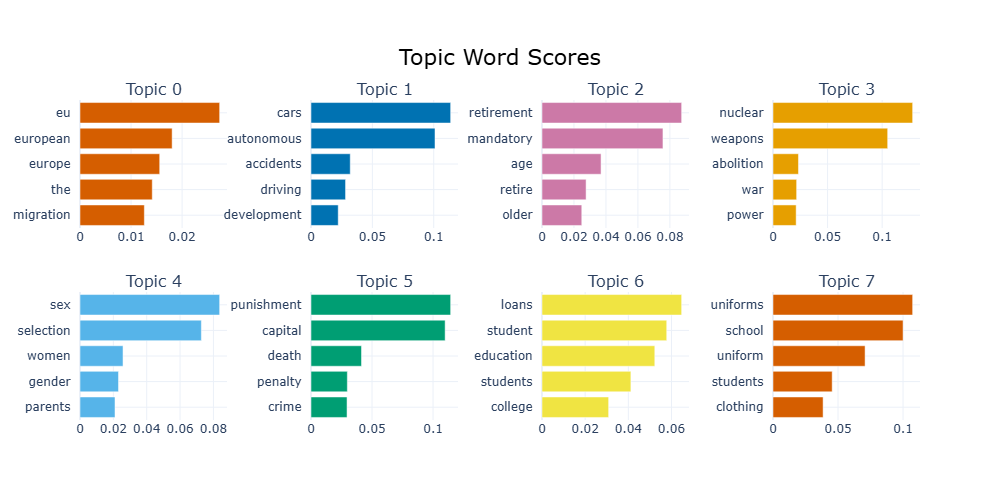
\includegraphics[width=0.9\linewidth,keepaspectratio]{images/results/topicmodeling/topic_word_scores.png}
%  \caption{Topic word scores for selected clusters (higher bars indicate higher c-TF--IDF weight).}
%  \label{fig:topic_word_scores}
%\end{figure}
%
%% --- Intertopic distance map image ---
%\begin{figure}[htbp]
%  \centering
%  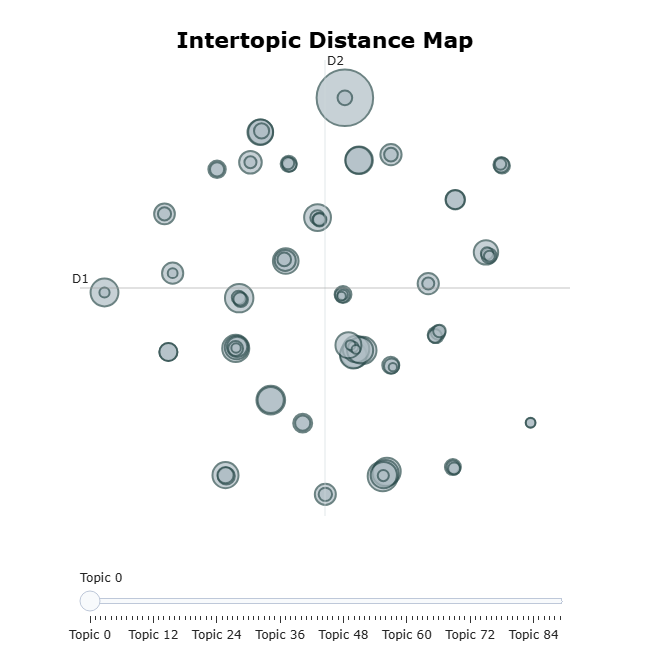
\includegraphics[width=0.9\linewidth,keepaspectratio]{images/results/topicmodeling/intertopic_distance_map.png}
%  \caption{Intertopic distance map from BERTopic showing relative topic positions and sizes.}
%  \label{fig:intertopic_distance}
%\end{figure}


\section{Agreement Ratio Analysis}

In this section we report the agreement ratios for each of the eight selected topics, across models (GPT, LLaMA) and prompting conditions (role-based, native). Each figure shows how often the model’s stance matched the gold stance for each country role, including the neutral assistant baseline.

\paragraph{General patterns.}
\begin{itemize}
    \item The \textbf{assistant baseline} is generally stable across topics and often lies in the mid-range of agreement ratios.
    \item \textbf{GPT} tends to be more consistent across roles and languages, with smaller gaps between conditions.
    \item \textbf{LLaMA} shows larger variability: in some topics, its agreement ratios diverge widely across roles or between role-based and native prompts.
    \item The magnitude of the \textbf{role vs.\ native difference} is topic-dependent: for some (e.g., prostitution, multi-party system) the results are close, while for others (e.g., sanctions, atheism) the divergence is large.
\end{itemize}

\paragraph{Topic-wise observations.}
\begin{itemize}
    \item \textbf{No nuclear weapons} 

    \begin{figure}[H]
    \centering
    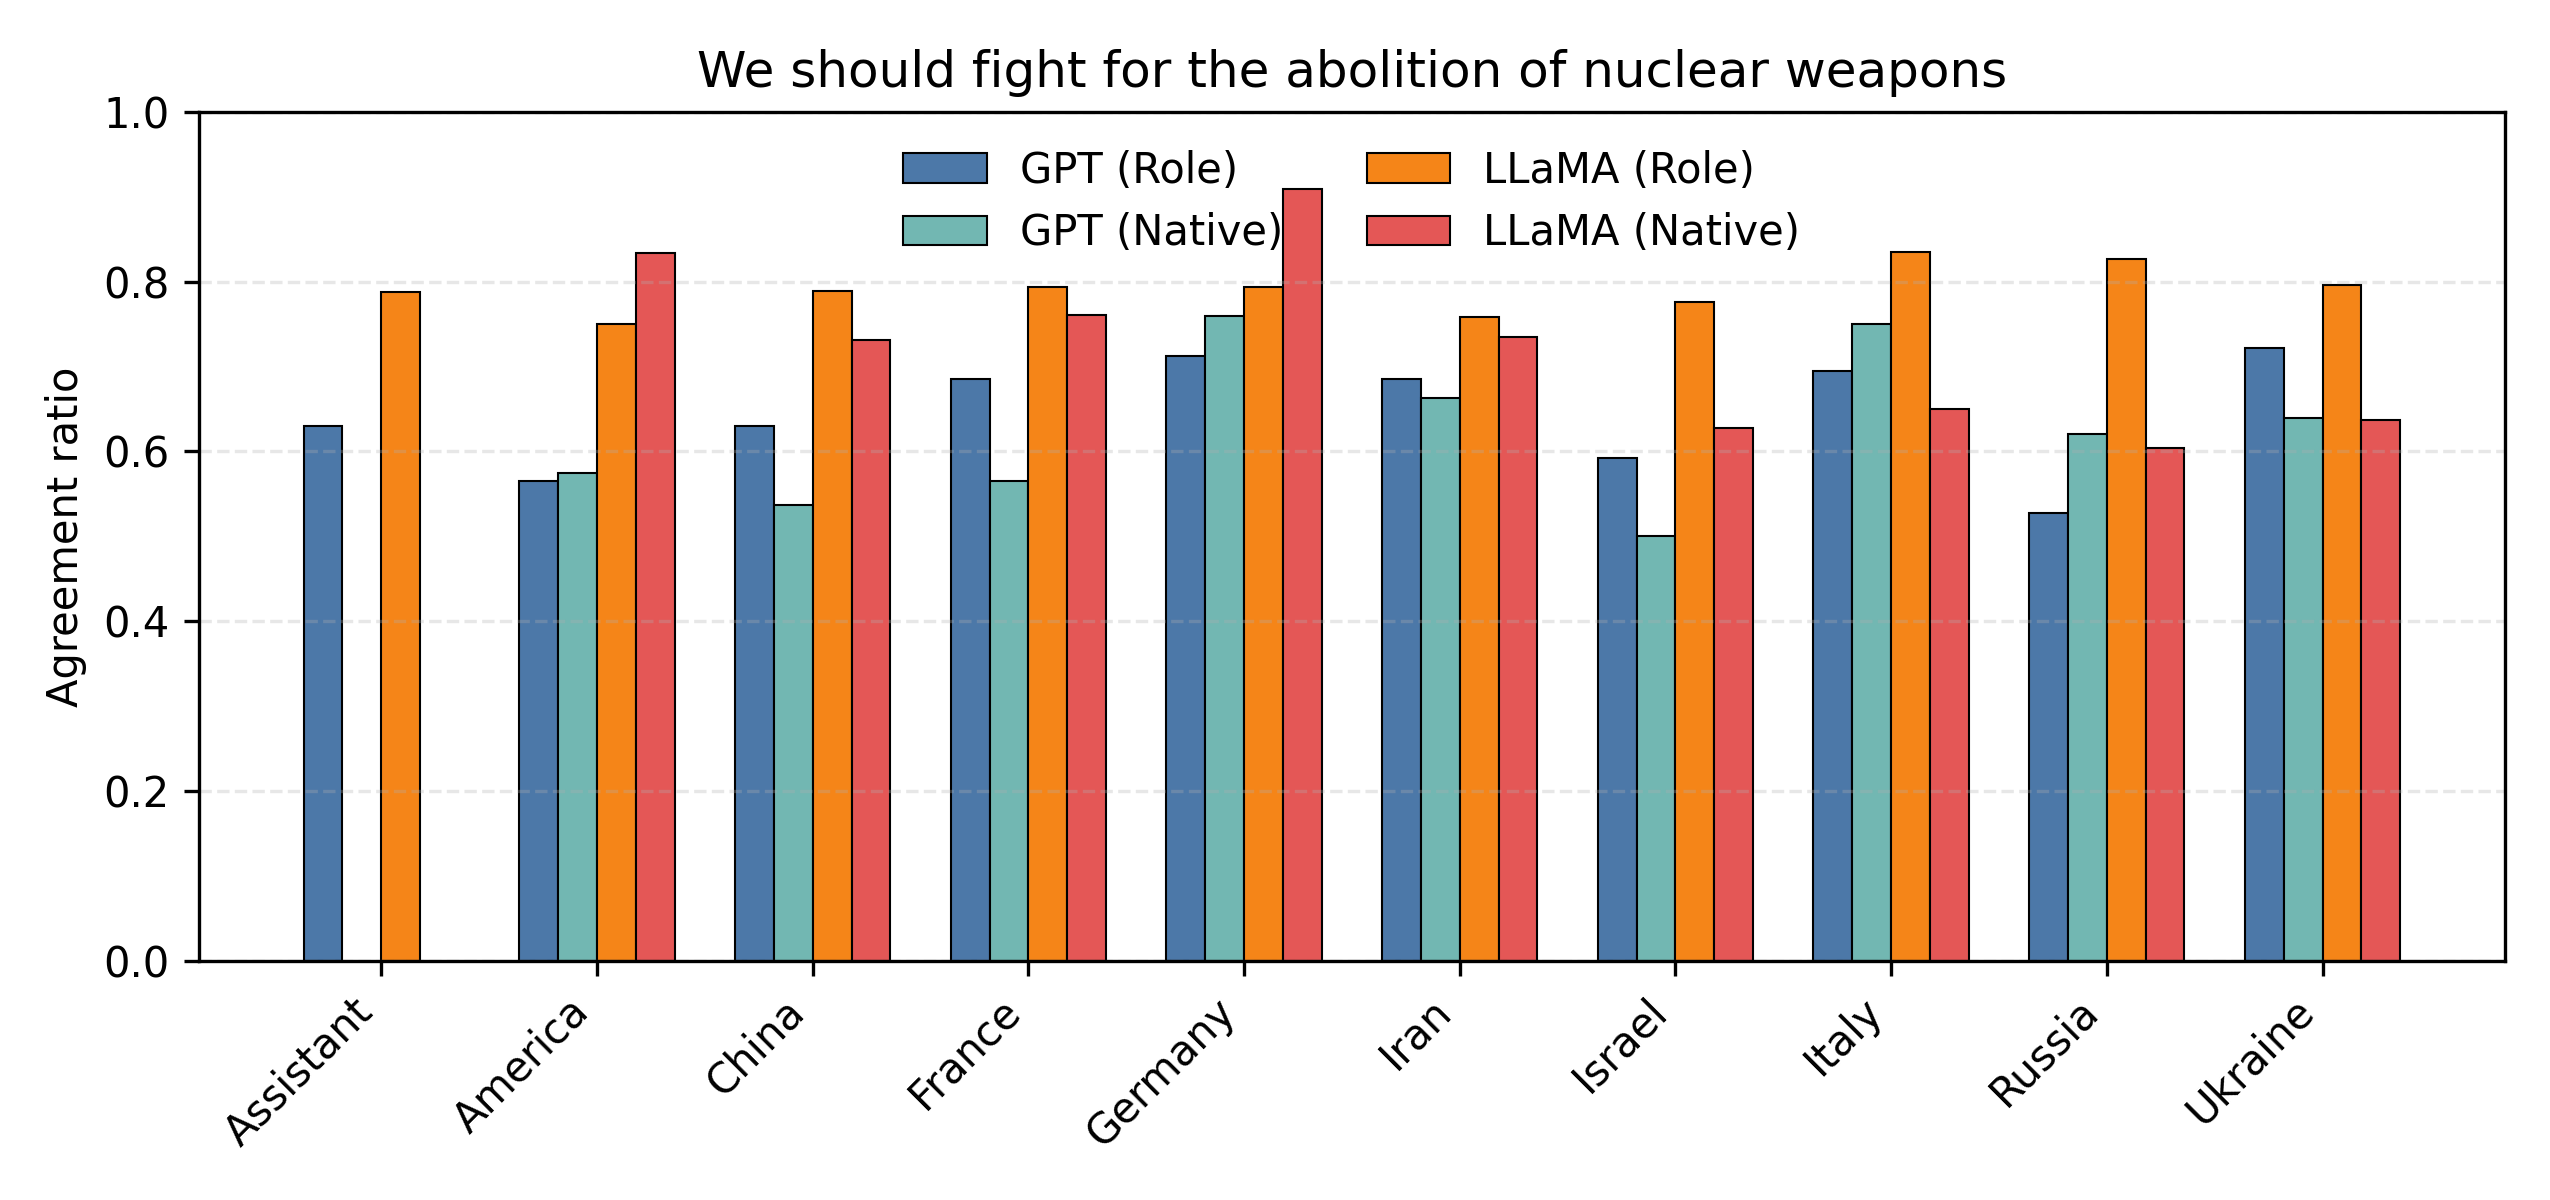
\includegraphics[width=0.85\textwidth]{images/results/agreement_ratio/agreement_topic_3_by_country}
    \caption{Agreement ratios by country for the topic ``No nuclear weapons.''}
    \label{fig:agreement_topic_3_by_country}
    \end{figure}
    
    (Figure~\ref{fig:agreement_topic_3_by_country}):  
    GPT produces agreement ratios around 0.6–0.8 with limited role/native spread. LLaMA is more variable, especially for Iran and Germany. Role vs.\ native differences are moderate.
    
    \item \textbf{Legalize sex selection} 

    \begin{figure}[H]
    \centering
    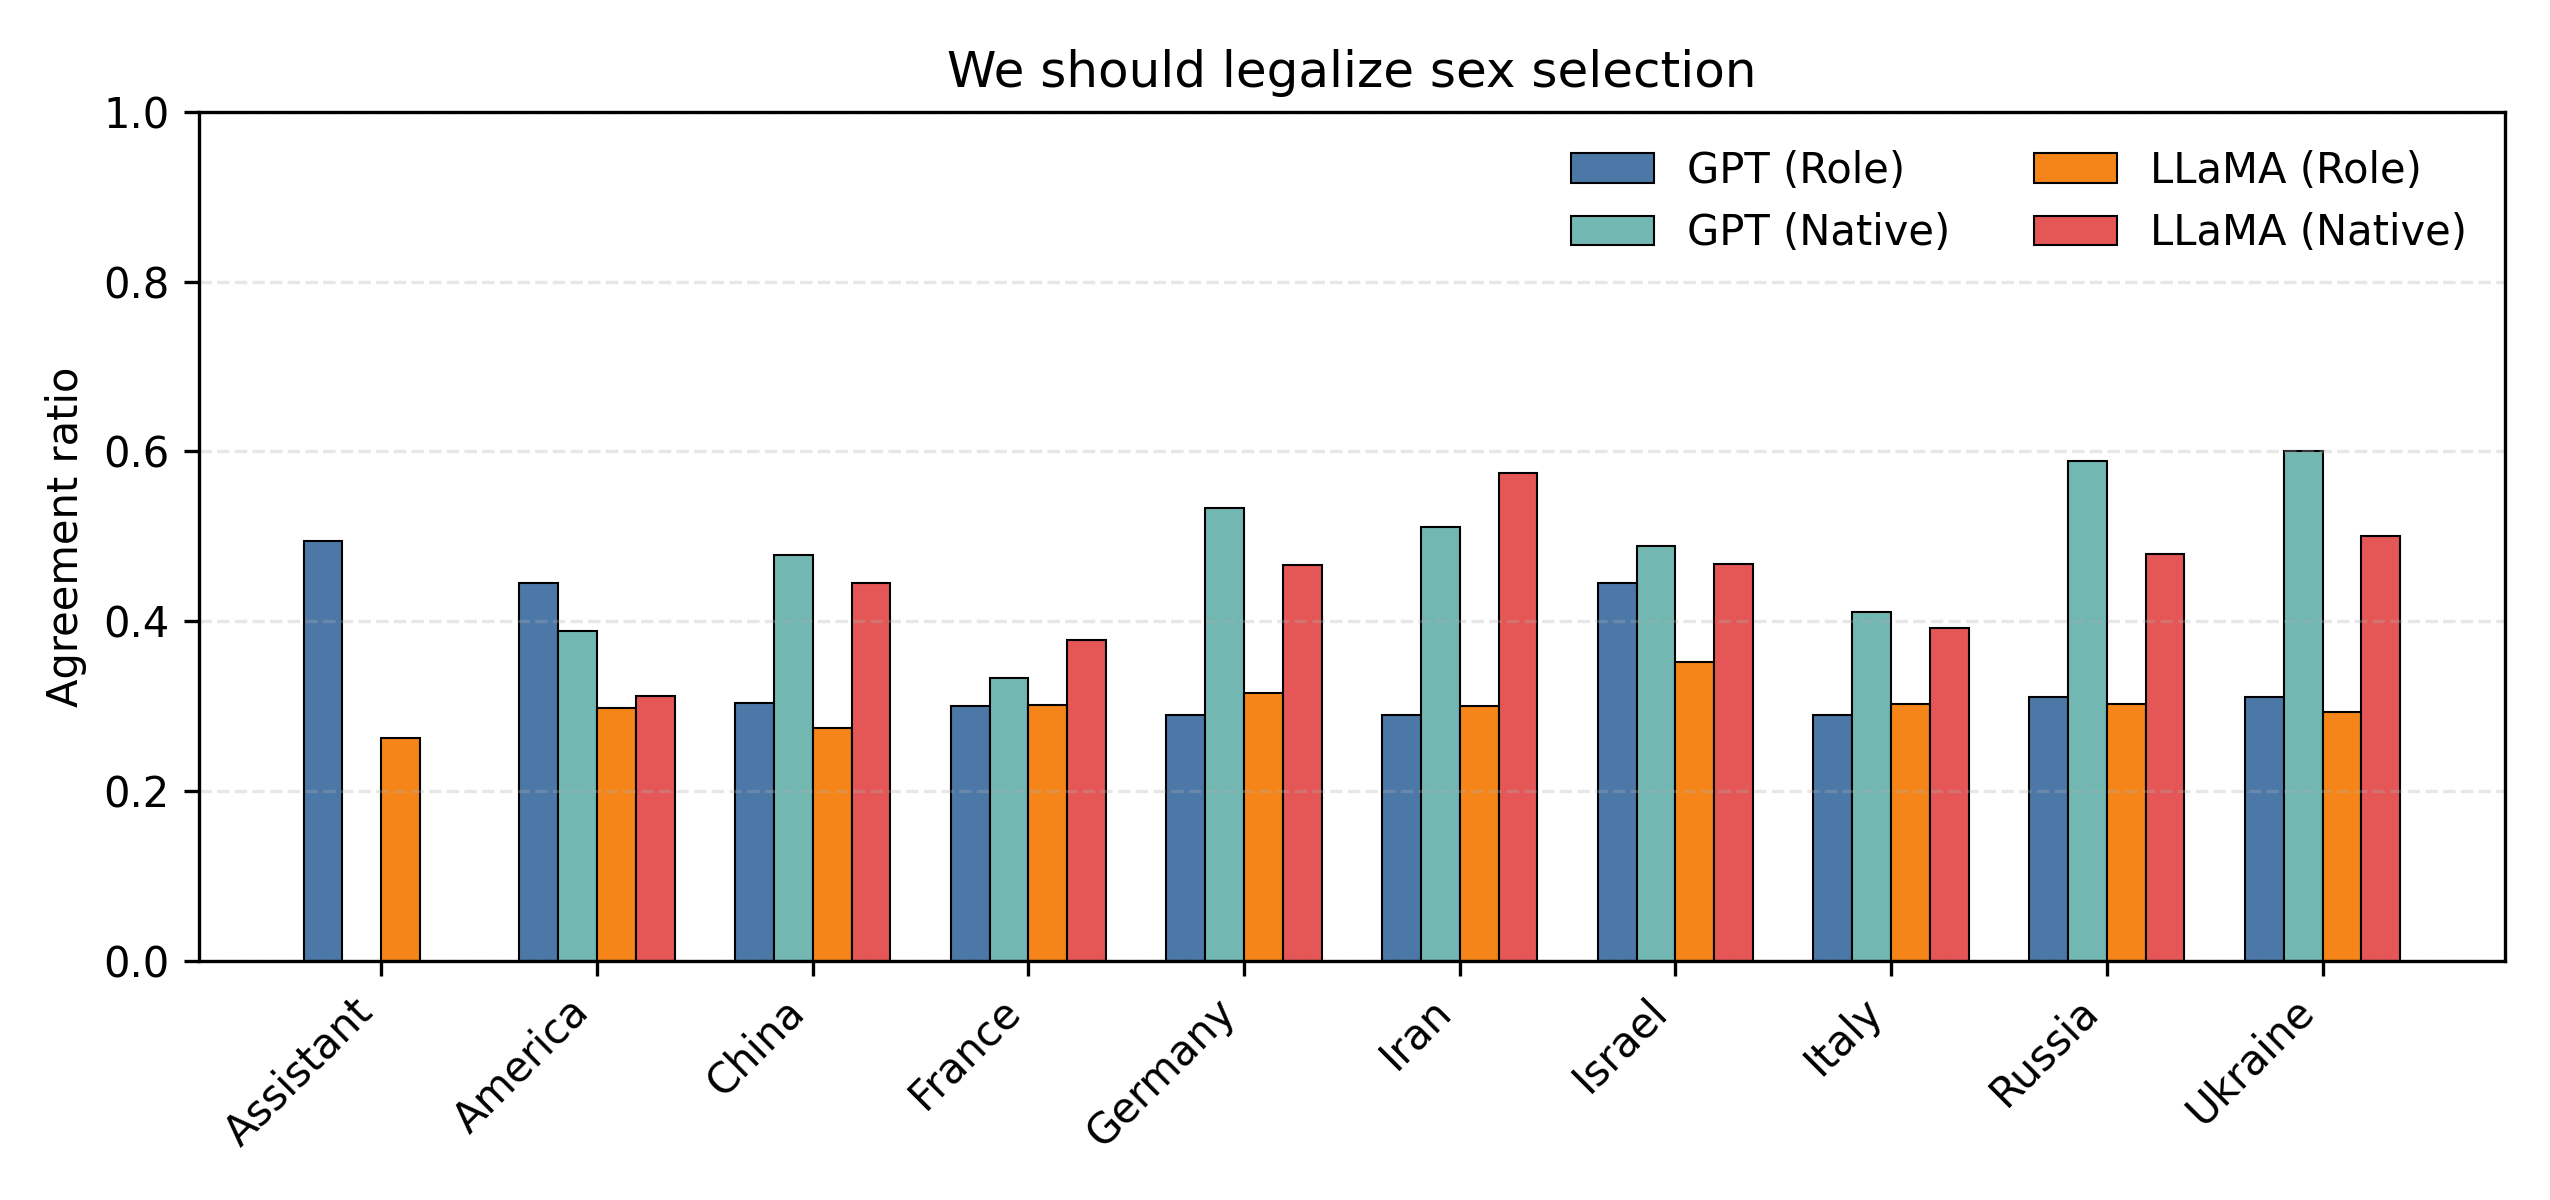
\includegraphics[width=0.85\textwidth]{images/results/agreement_ratio/agreement_topic_4_by_country}
    \caption{Agreement ratios by country for the topic ``Legalize sex selection.''}
    \label{fig:agreement_topic_4_by_country}
    \end{figure}
    
    (Figure~\ref{fig:agreement_topic_4_by_country}):  
    Both models lean toward disagreement (ratios often below 0.5). Larger role/native gaps appear in some countries (e.g., Iran, China).
    
    \item \textbf{No economic sanctions} 
    
    \begin{figure}[H]
    \centering
    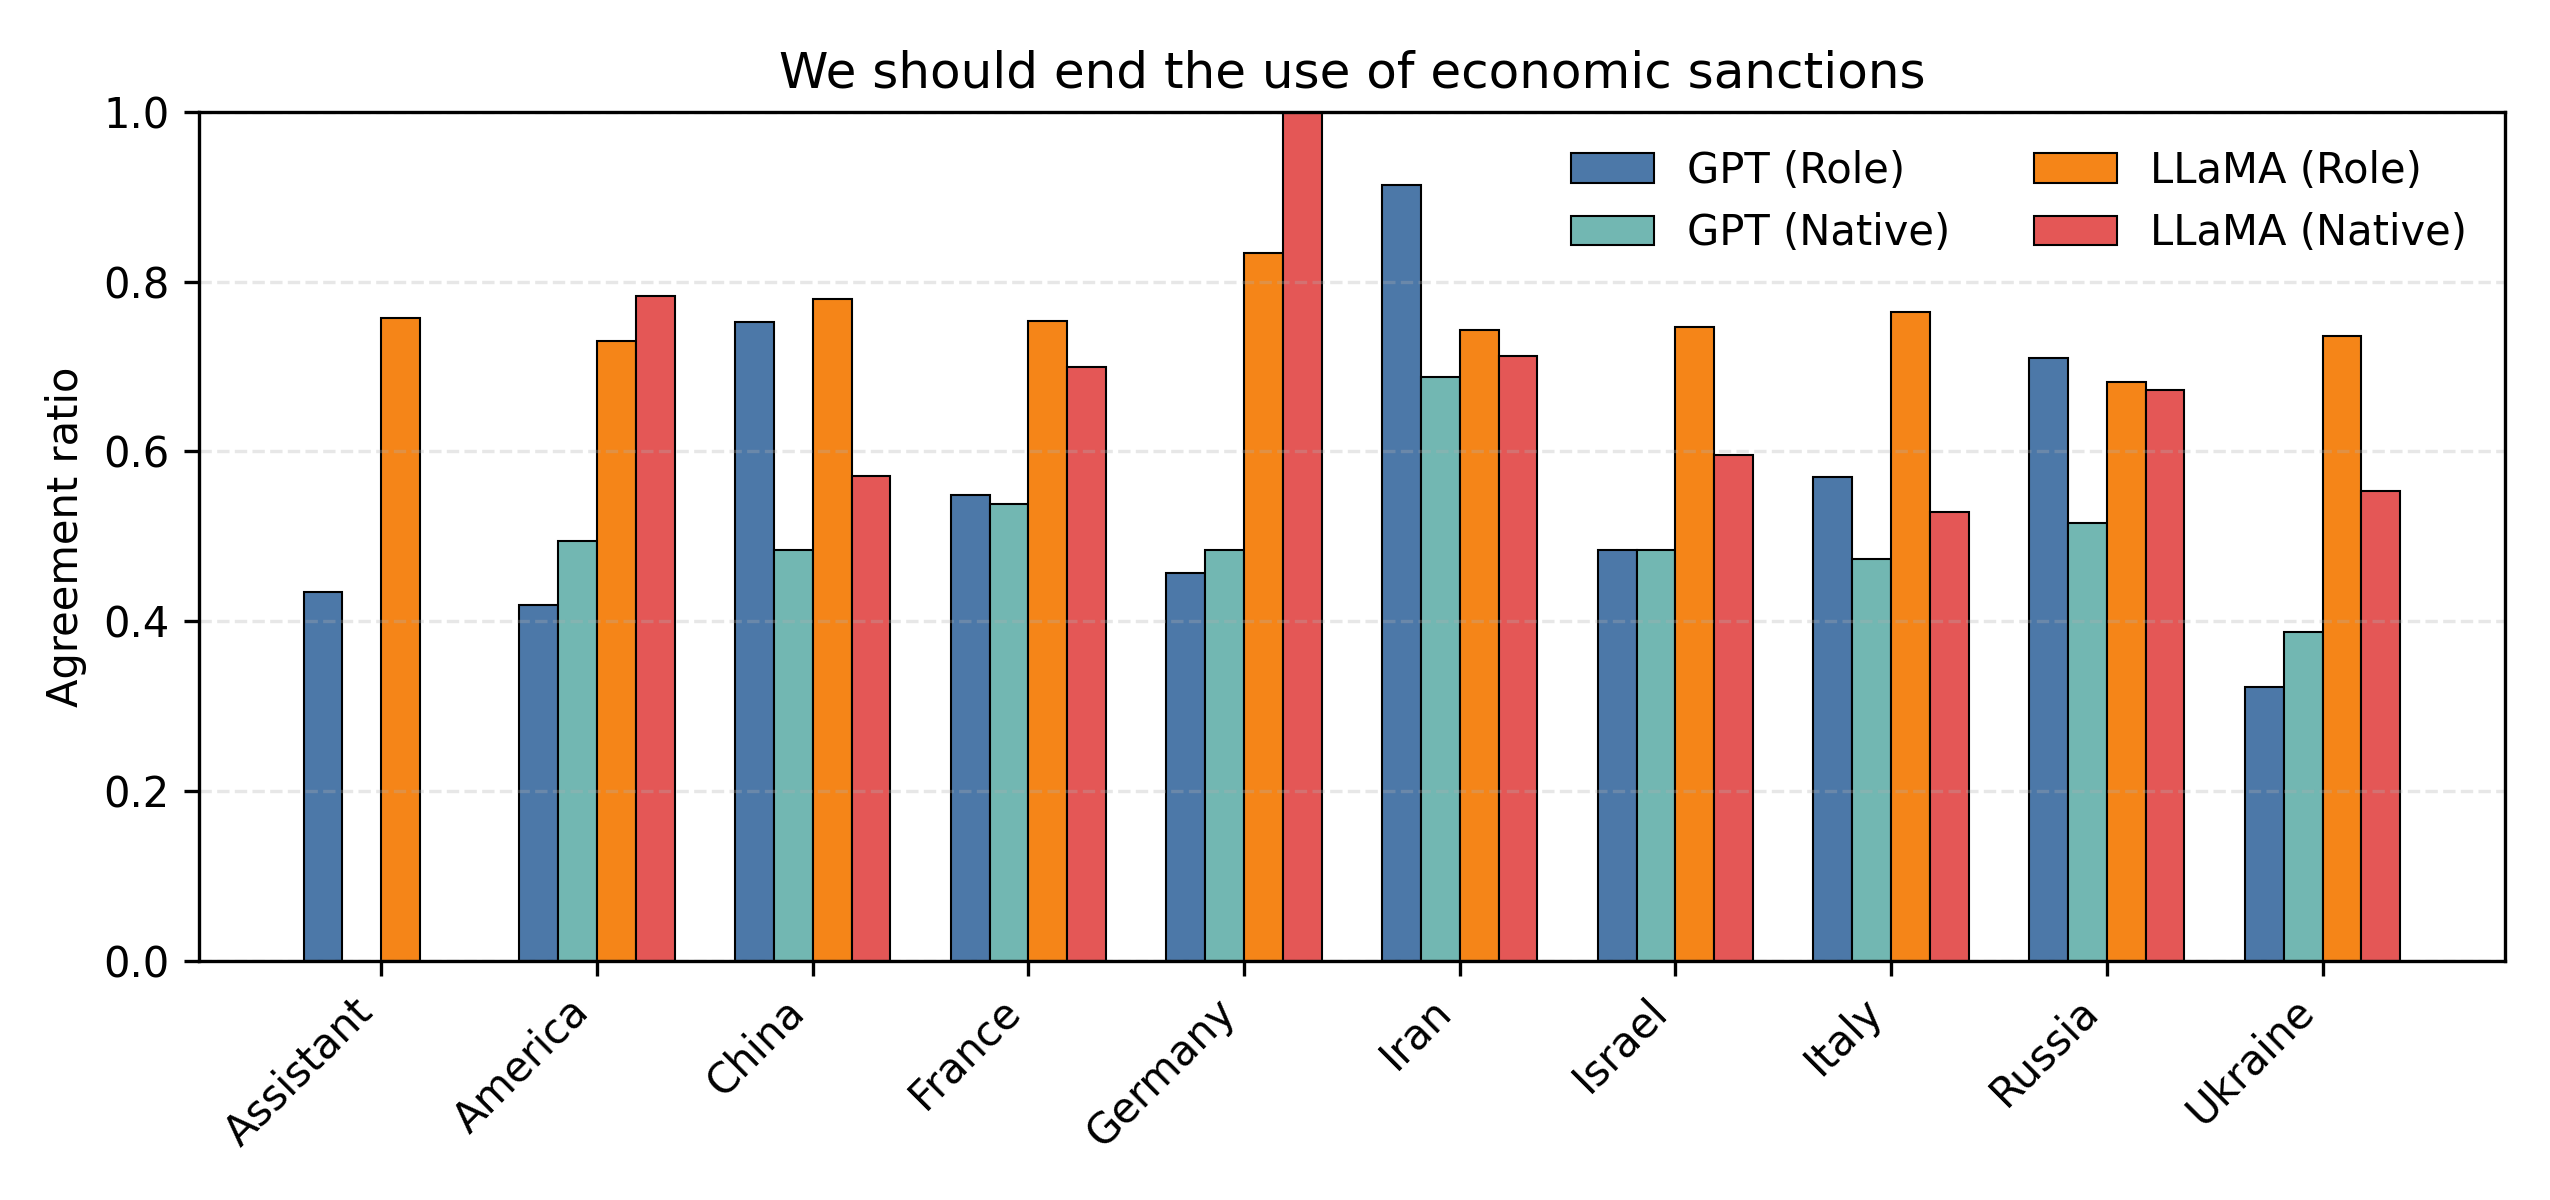
\includegraphics[width=0.85\textwidth]{images/results/agreement_ratio/agreement_topic_15_by_country}
    \caption{Agreement ratios by country for the topic ``No economic sanctions.''}
    \label{fig:agreement_topic_15_by_country}
    \end{figure}
    
    (Figure~\ref{fig:agreement_topic_15_by_country}):  
    Strong divergences. GPT remains in the 0.4–0.7 range, while LLaMA peaks close to 0.9 for Iran (role-based). Role/native gaps are particularly large in LLaMA.
    
    \item \textbf{Legalize prostitution} 

    \begin{figure}[H]
    \centering
    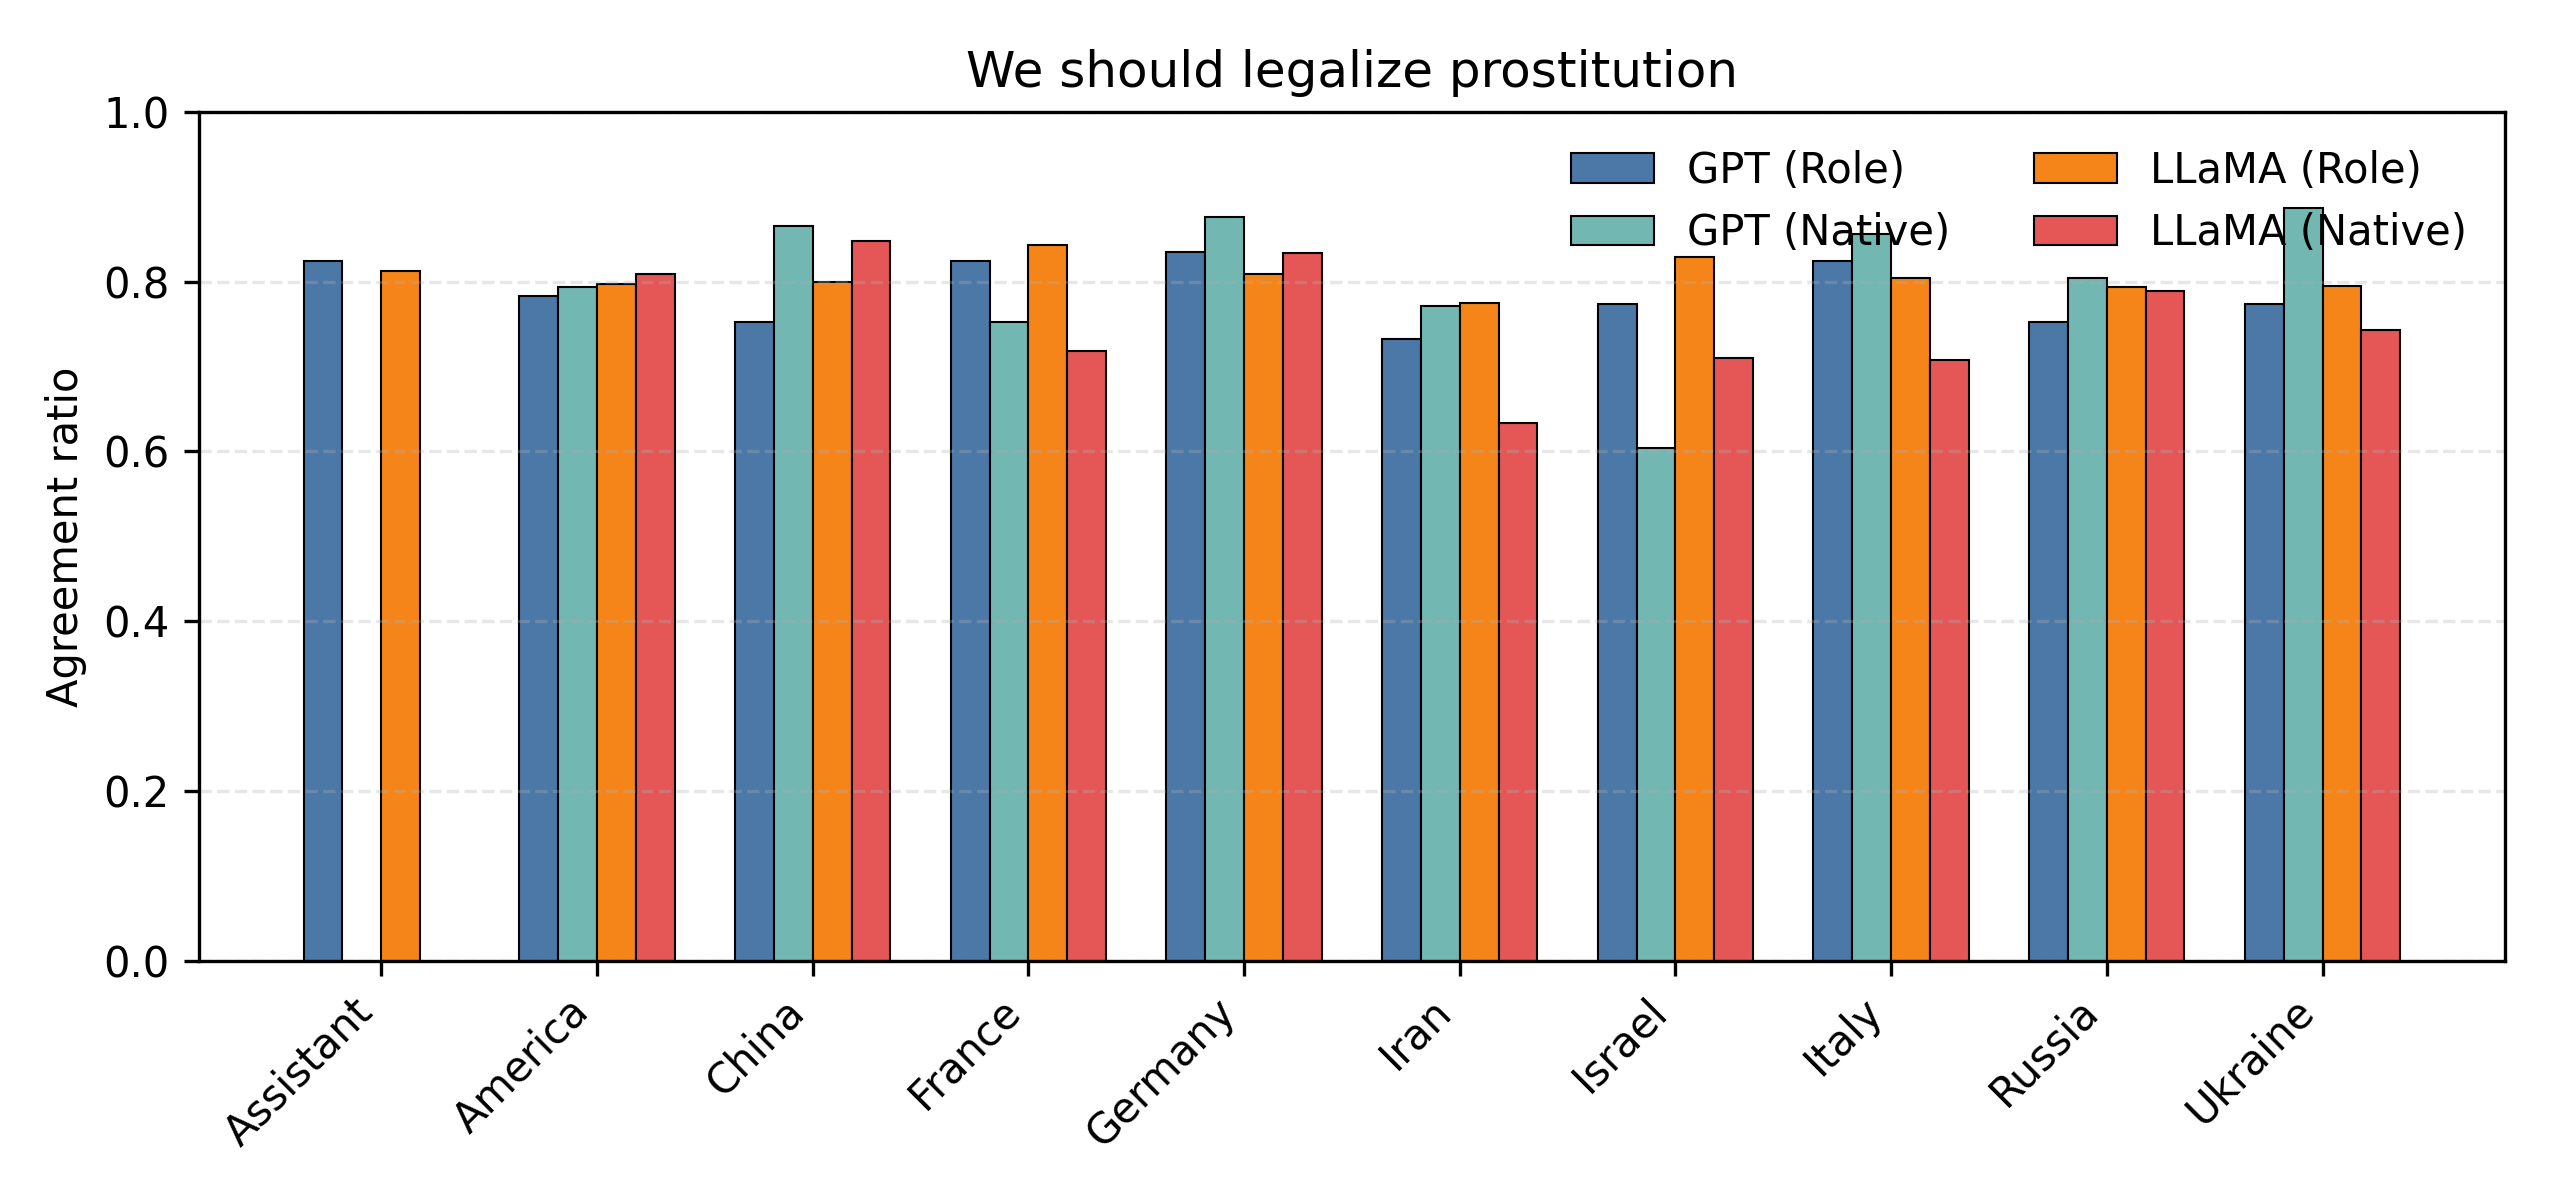
\includegraphics[width=0.85\textwidth]{images/results/agreement_ratio/agreement_topic_17_by_country}
    \caption{Agreement ratios by country for the topic ``Legalize prostitution.''}
    \label{fig:agreement_topic_17_by_country}
    \end{figure}
    
    (Figure~\ref{fig:agreement_topic_17_by_country}):  
    High agreement ($>0.7$) across all models and conditions. Role vs.\ native differences are minimal.
    
    \item \textbf{Adopt multi-party system} 
    
    \begin{figure}[H]
    \centering
    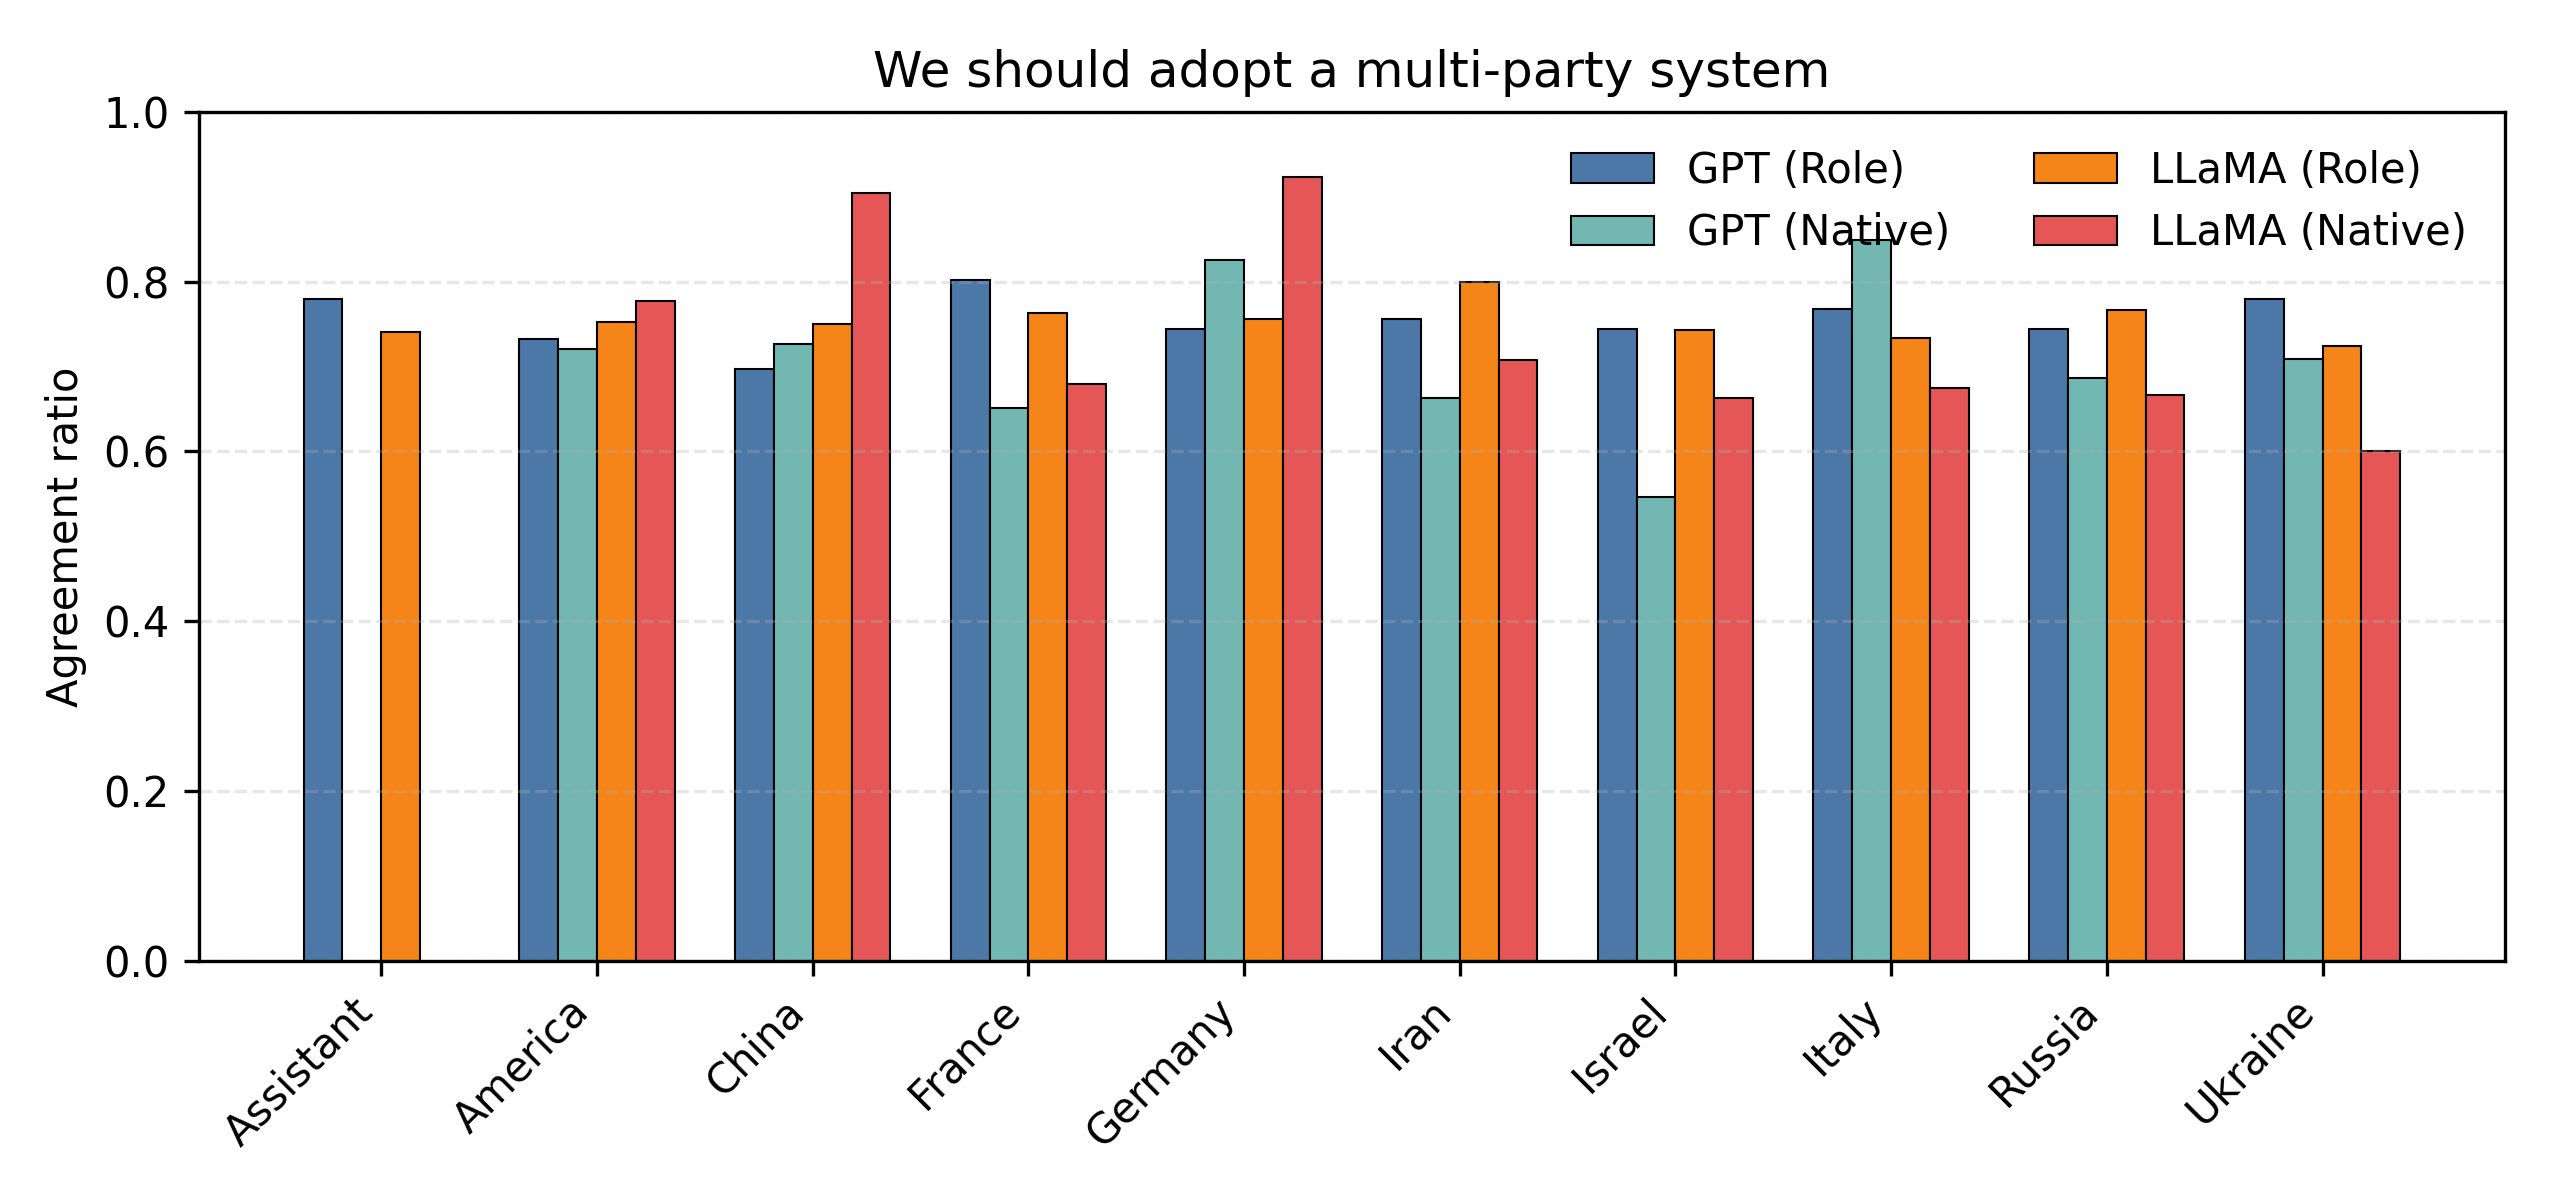
\includegraphics[width=0.85\textwidth]{images/results/agreement_ratio/agreement_topic_18_by_country}
    \caption{Agreement ratios by country for the topic ``Adopt multi-party system.''}
    \label{fig:agreement_topic_18_by_country}
    \end{figure}
    
    (Figure~\ref{fig:agreement_topic_18_by_country}):  
    Both models yield high agreement (0.7–0.9). Role and native completions are closely aligned, with little divergence.
    
    \item \textbf{Adopt atheism} 

    \begin{figure}[H]
    \centering
    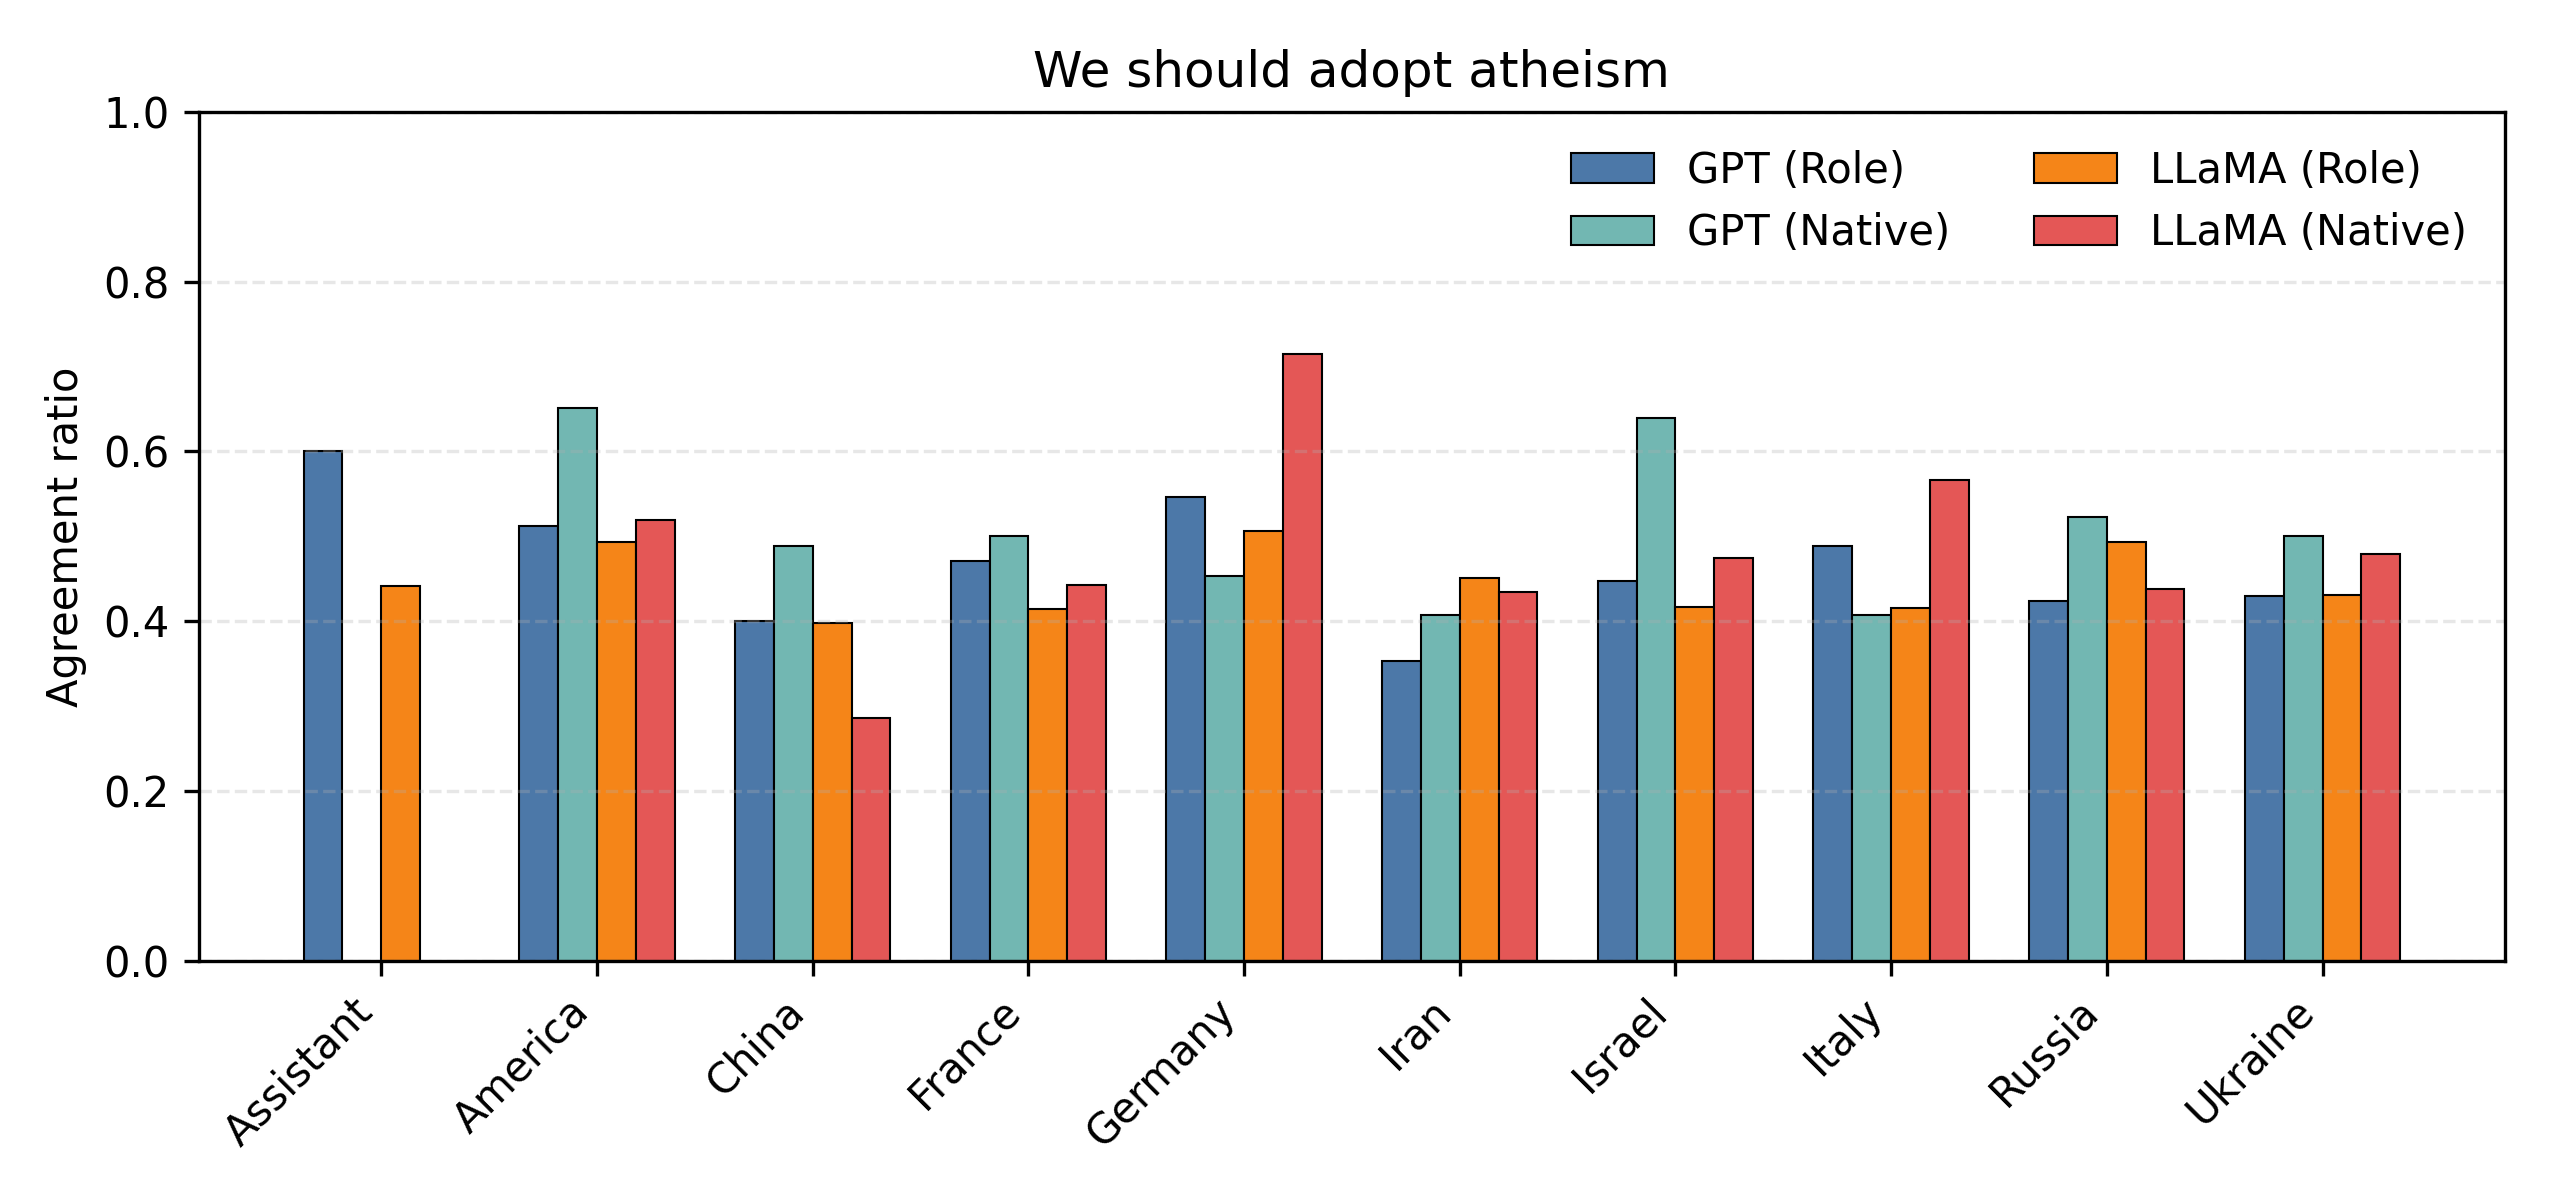
\includegraphics[width=0.85\textwidth]{images/results/agreement_ratio/agreement_topic_22_by_country}
    \caption{Agreement ratios by country for the topic ``Adopt atheism.''}
    \label{fig:agreement_topic_22_by_country}
    \end{figure}
    
    (Figure~\ref{fig:agreement_topic_22_by_country}):  
    Strong variation across roles and models. GPT tends to remain below 0.6, while LLaMA shows higher spread and larger role/native gaps. Divergences are particularly marked in countries with religious framing.
    
    \item \textbf{Compulsory voting} 
    
    \begin{figure}[H]
    \centering
    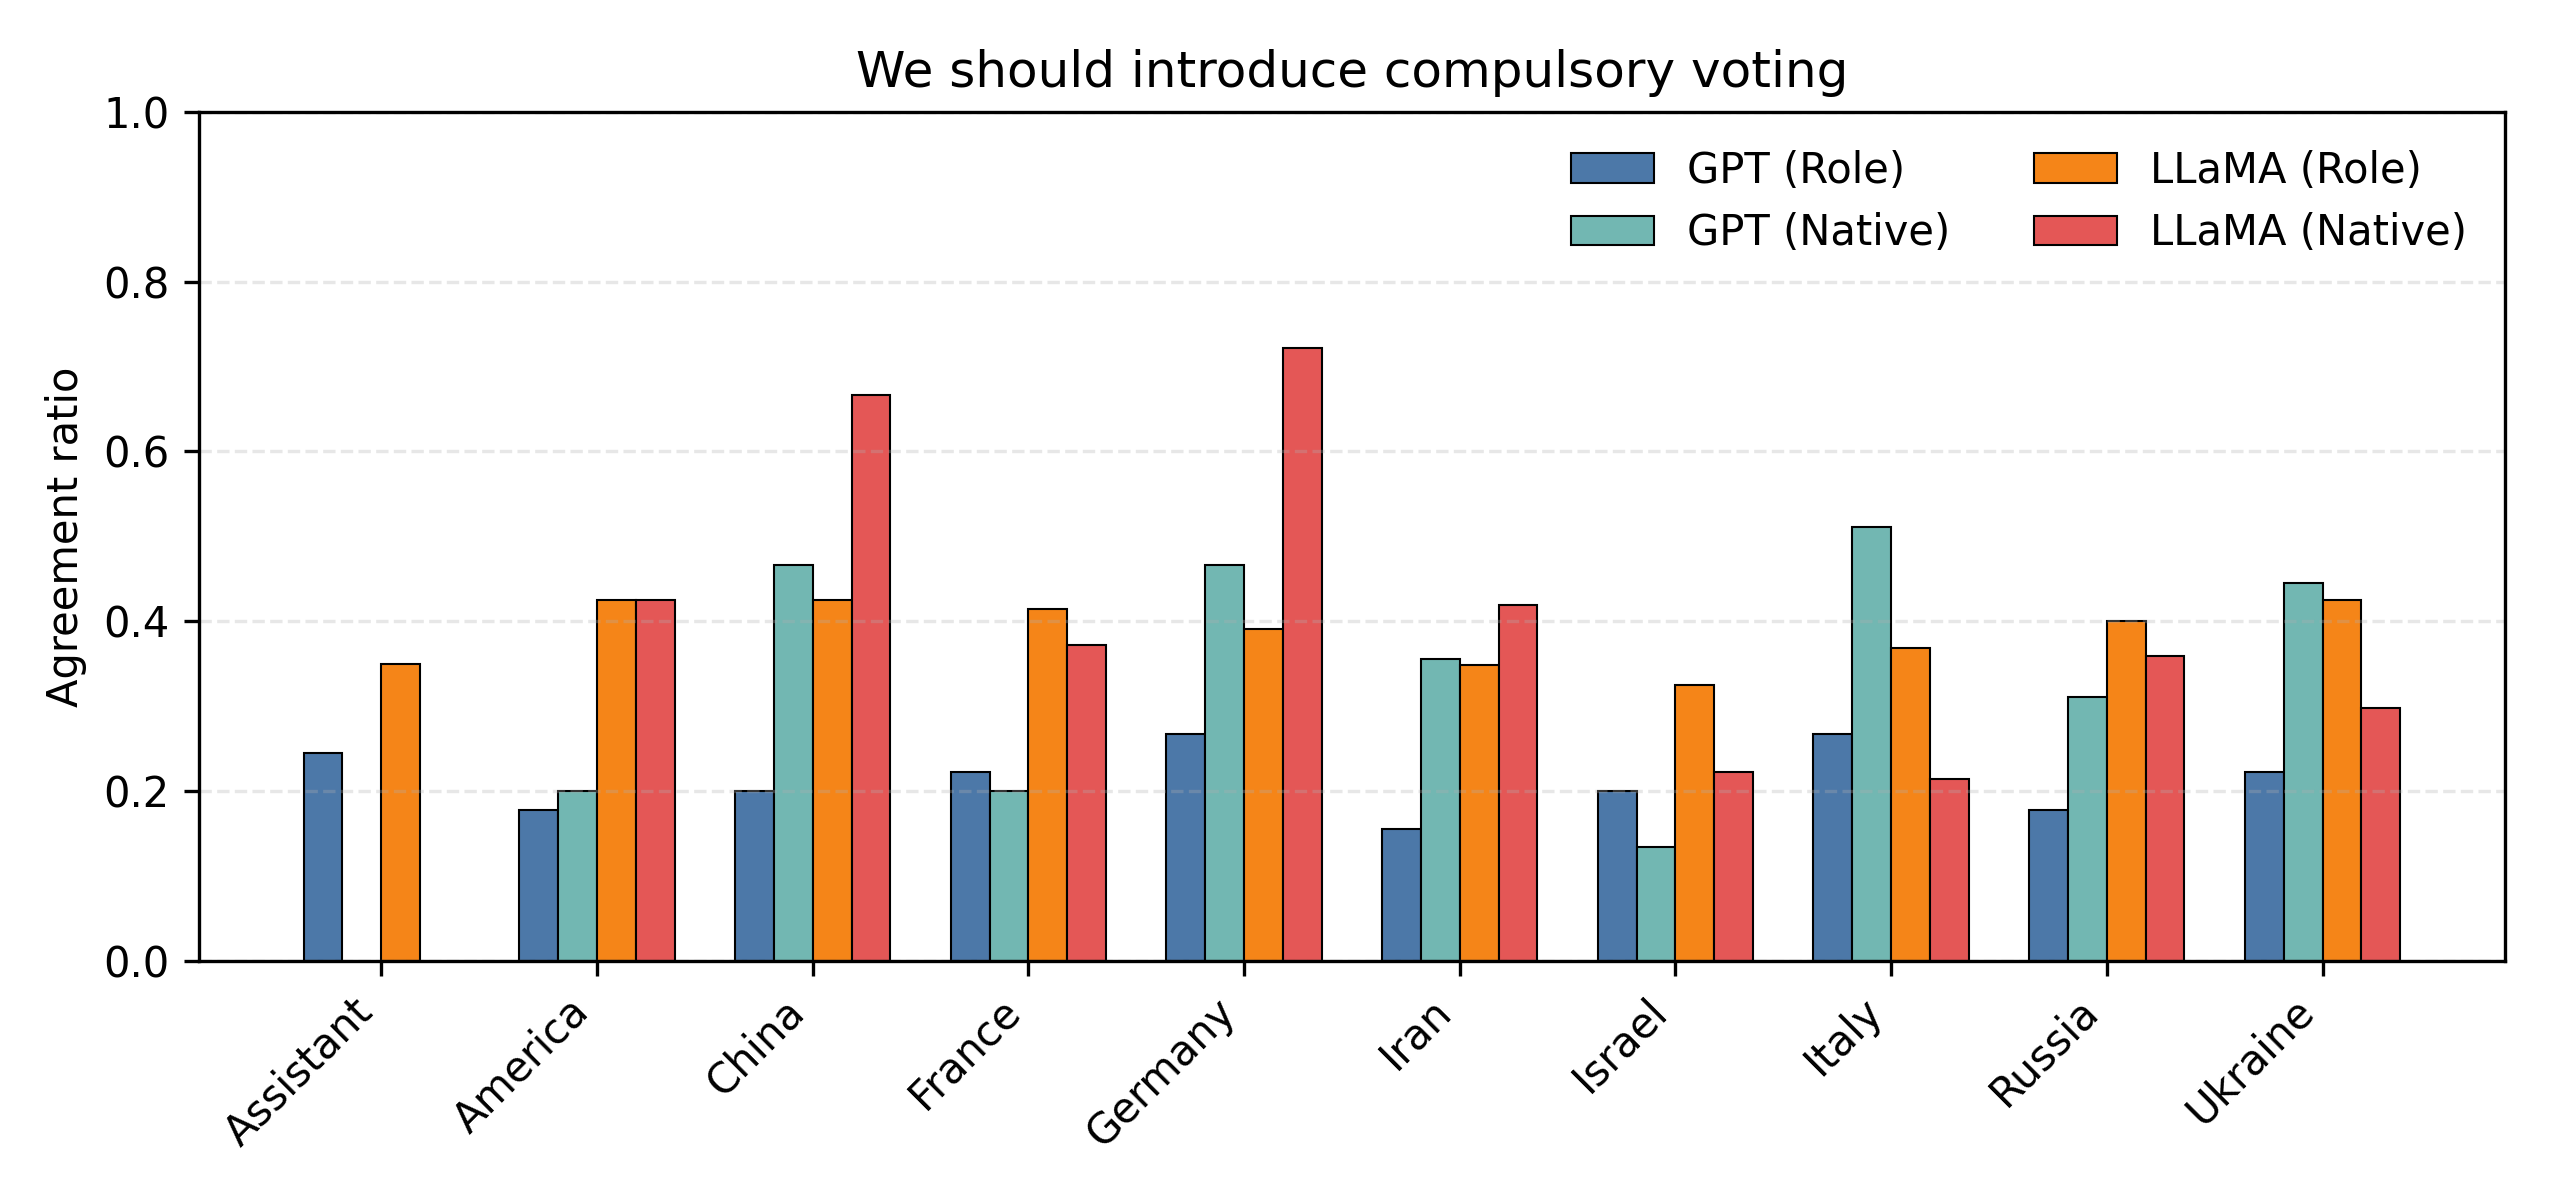
\includegraphics[width=0.85\textwidth]{images/results/agreement_ratio/agreement_topic_36_by_country}
    \caption{Agreement ratios by country for the topic ``Compulsory voting.''}
    \label{fig:agreement_topic_36_by_country}
    \end{figure}
    
    (Figure~\ref{fig:agreement_topic_36_by_country}):  
    The lowest agreement ratios overall. GPT mostly falls around 0.2–0.4, while LLaMA ranges more widely, with some roles exceeding 0.6. Role/native divergence is higher than in most other topics.
    
    \item \textbf{Adopt libertarianism} 
    
    \begin{figure}[H]
    \centering
    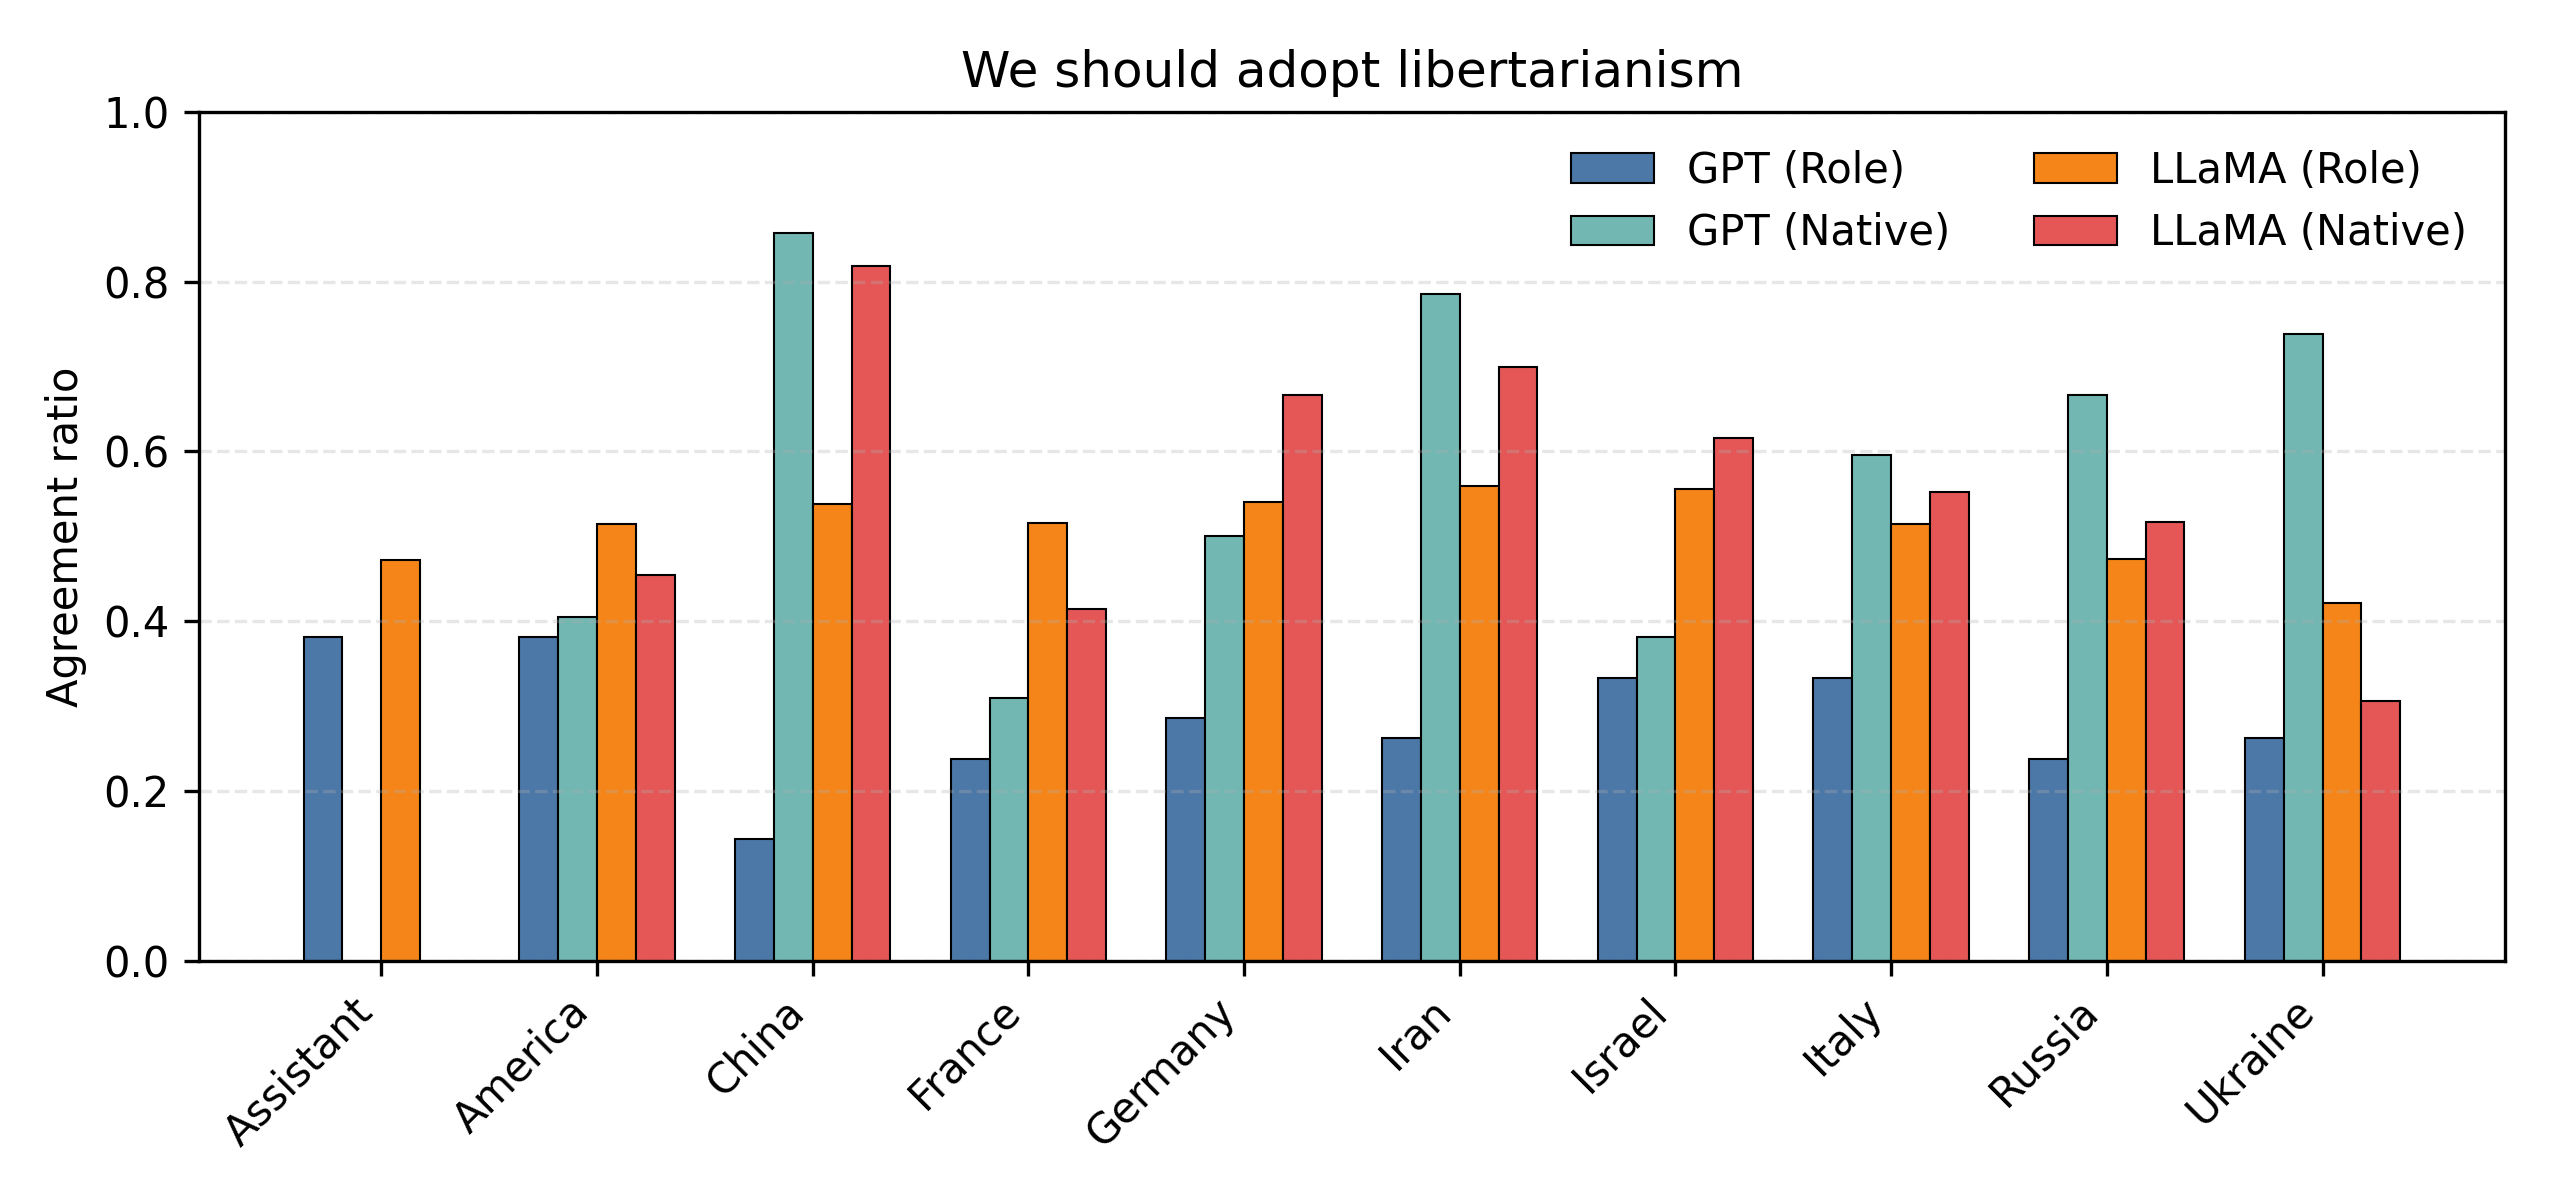
\includegraphics[width=0.85\textwidth]{images/results/agreement_ratio/agreement_topic_40_by_country}
    \caption{Agreement ratios by country for the topic ``Adopt libertarianism.''}
    \label{fig:agreement_topic_40_by_country}
    \end{figure}
    
    (Figure~\ref{fig:agreement_topic_40_by_country}):  
    Mid-range ratios (0.4–0.7). Both models show noticeable differences between role and native completions, though the size of the gap varies across countries.
\end{itemize}

\paragraph{Summary.}
Across topics, GPT demonstrates more stable agreement ratios with smaller role/native differences, while LLaMA exhibits stronger variability. Topics such as \emph{prostitution} and \emph{multi-party system} are consistently aligned across conditions, whereas \emph{sanctions}, \emph{atheism}, and \emph{compulsory voting} show the largest divergences.


%========================================================
% Embedding similarities
% (Requires in preamble: \usepackage{graphicx,subcaption,booktabs,amsmath})
%========================================================
\section{Embedding similarities}
We quantify the semantic proximity between model justifications using mean cosine similarity across the eight topics (whiskers in the bar charts show \emph{standard deviation across topics}, i.e., topic dispersion, not confidence intervals). For each model we report three pairwise comparisons—\emph{Native vs. Role} (NvR), \emph{Role vs. Assistant} (RvA), and \emph{Native vs. Assistant} (NvA)—first as bar charts to capture global patterns by country, then as heatmaps to expose country–topic detail.

%---------------------------
\subsection{GPT-4o-mini}
%---------------------------

\paragraph{Bar-chart interpretation.}
As illustrated in Figure~\ref{fig:gpt_bars}, \emph{Persona $>$ language.} NvA and NvR are consistently higher than RvA for almost all countries (typically by a visible margin), indicating that role prompts reshape reasons more than switching language. NvA and NvR display modest topic dispersion, whereas RvA exhibits the largest dispersion—i.e., stronger topic dependence—most notably for China and several lower-scoring countries. Country ordering is stable: USA highest; Germany/France/Italy/Russia mid–high; China/Israel/Iran/Ukraine somewhat lower.

\begin{figure}[H]
  \centering
  % --- three bar charts (replace file paths with yours) ---
  \begin{subfigure}{.48\linewidth}
    \centering
    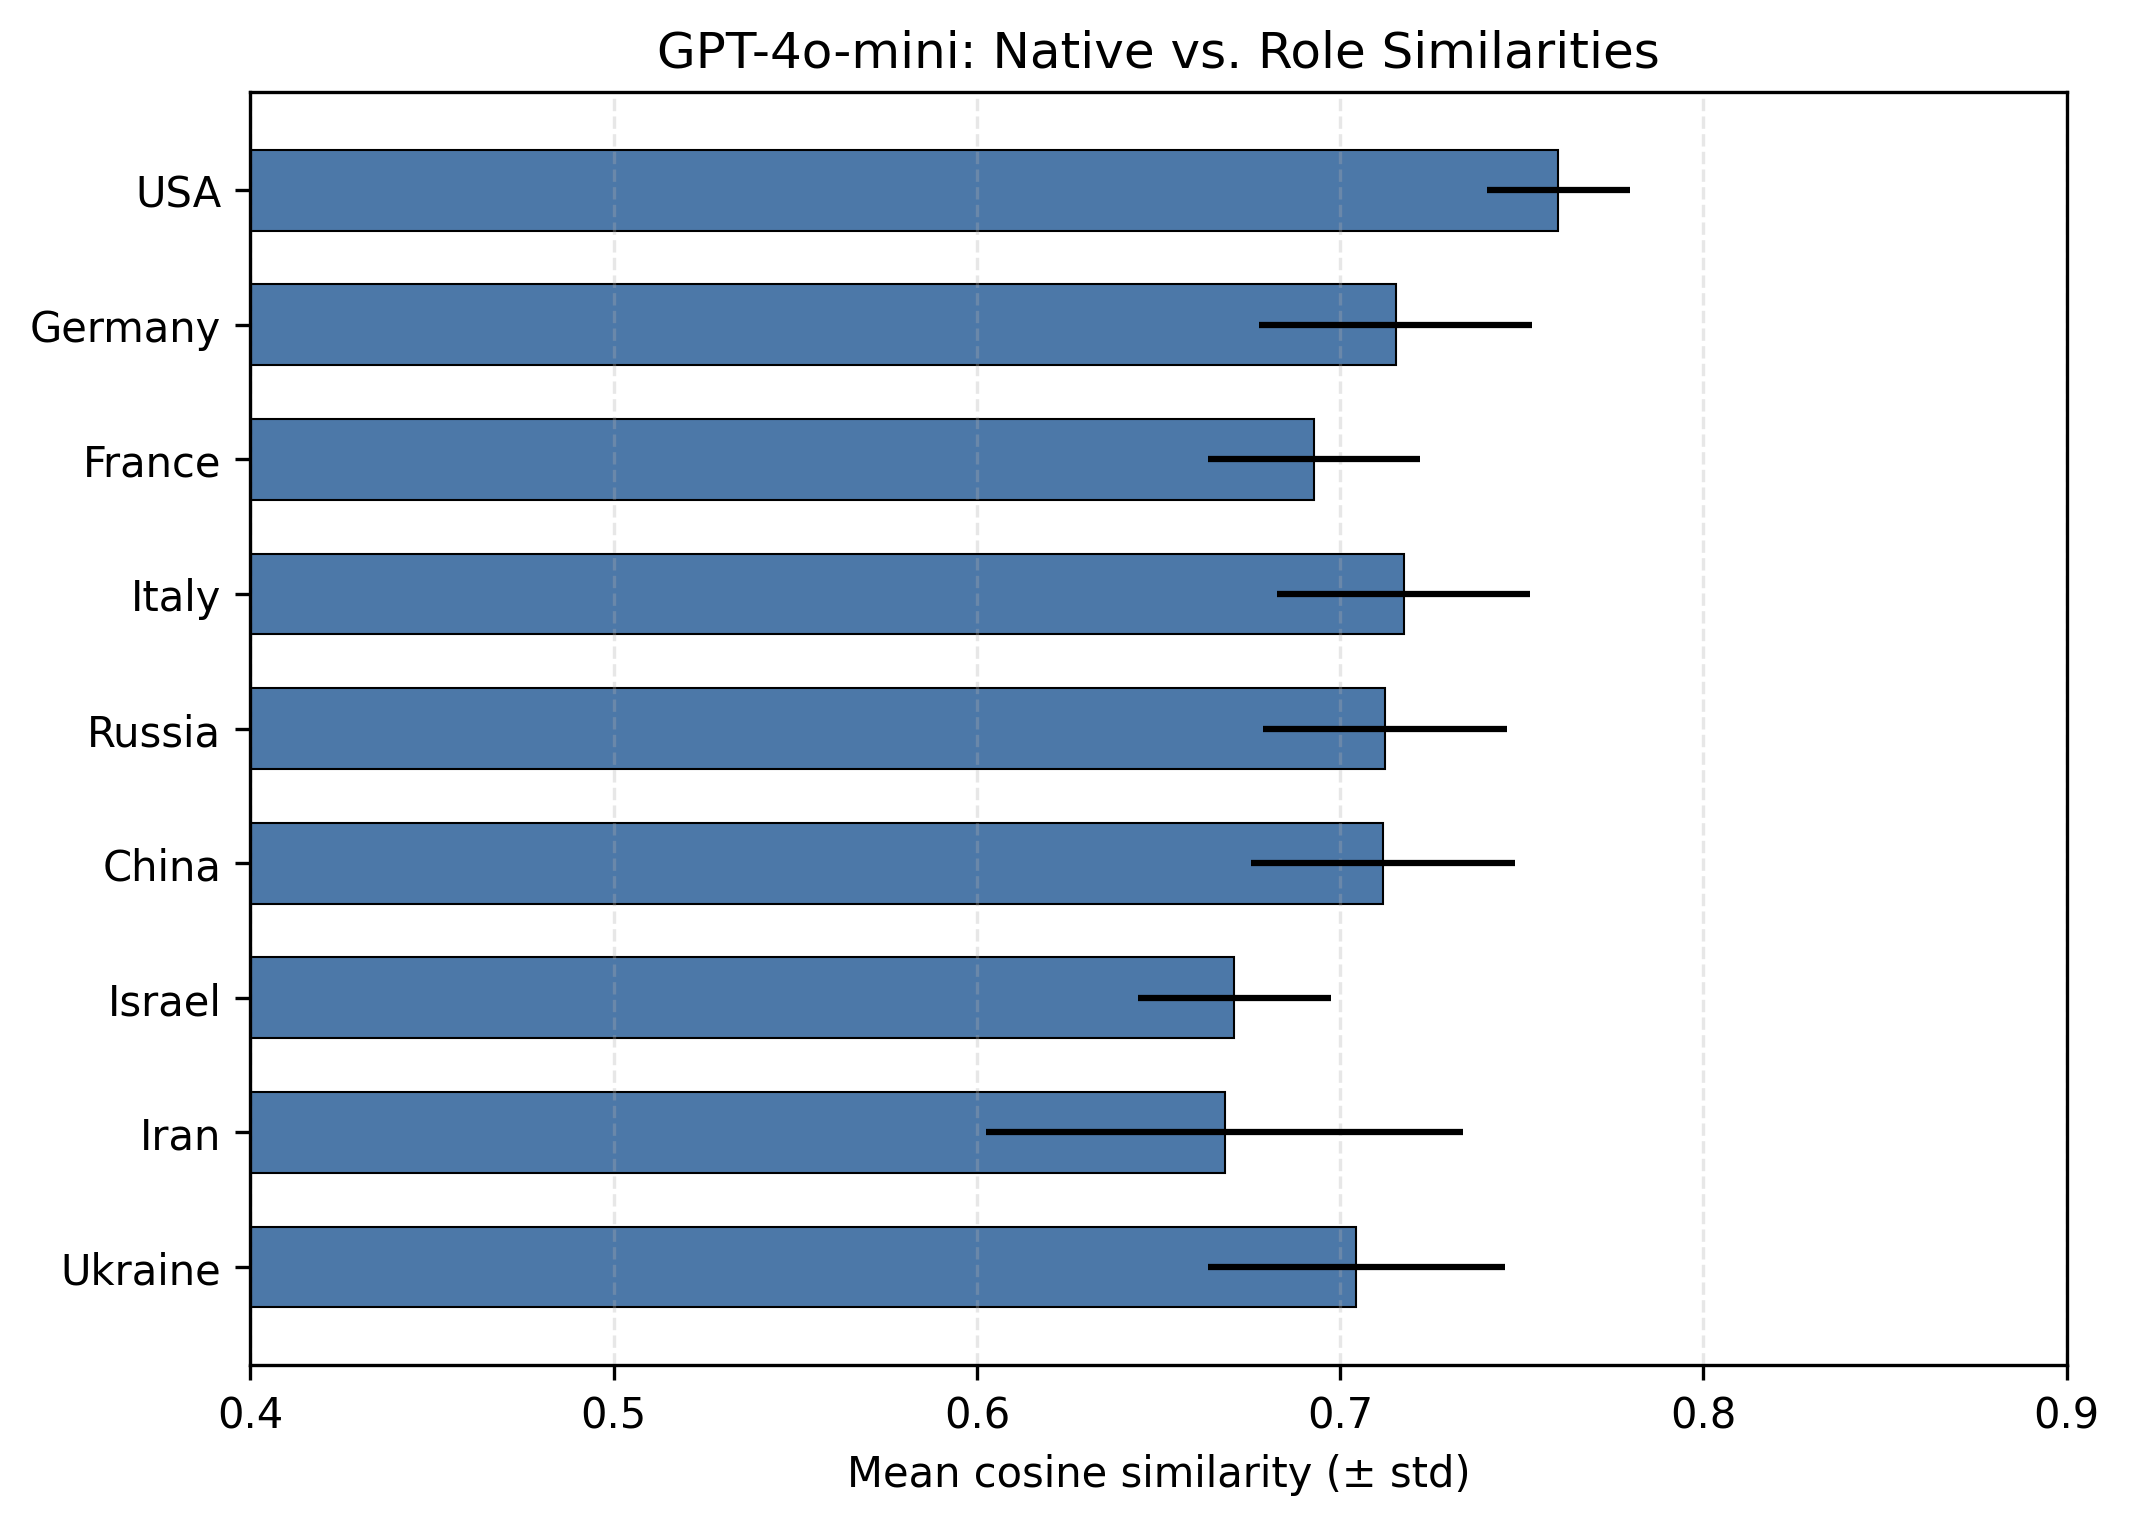
\includegraphics[width=\linewidth]{images/results/similarity/gpt/native_vs_role_summary}
    \caption{Native vs. Role (NvR)}
  \end{subfigure}\hfill
  \begin{subfigure}{.48\linewidth}
    \centering
    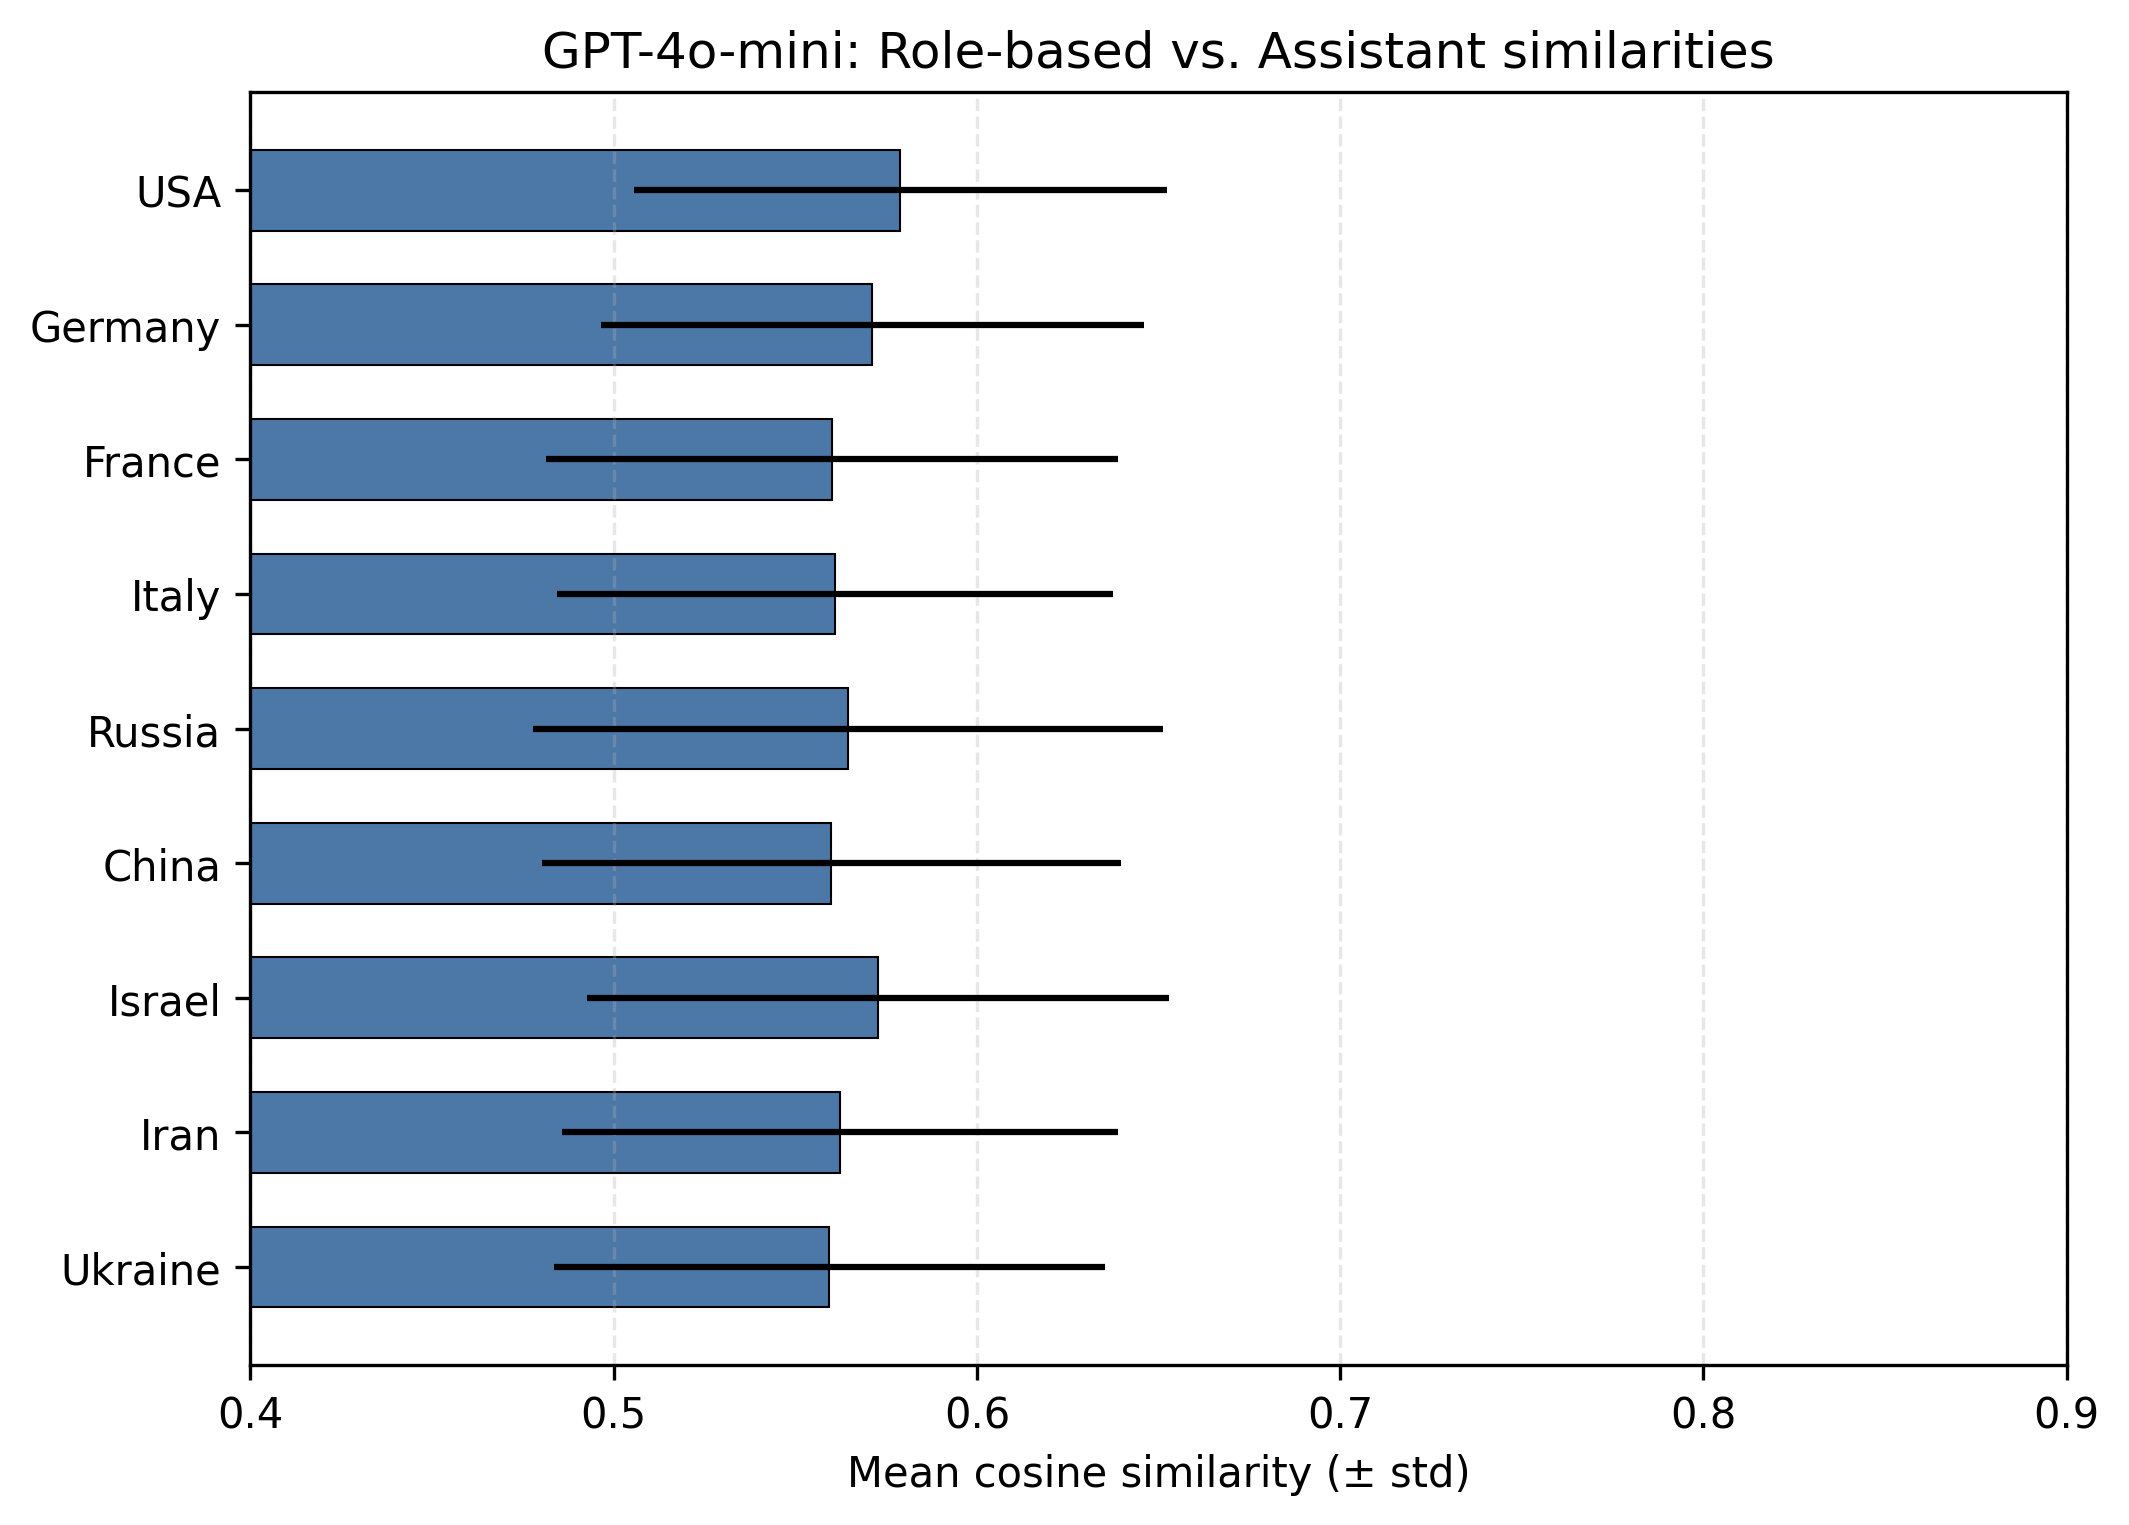
\includegraphics[width=\linewidth]{images/results/similarity/gpt/rolebased_vs_assistant_summary}
    \caption{Role vs. Assistant (RvA)}
  \end{subfigure}\\[0.75em]
  \begin{subfigure}{.48\linewidth}
    \centering
    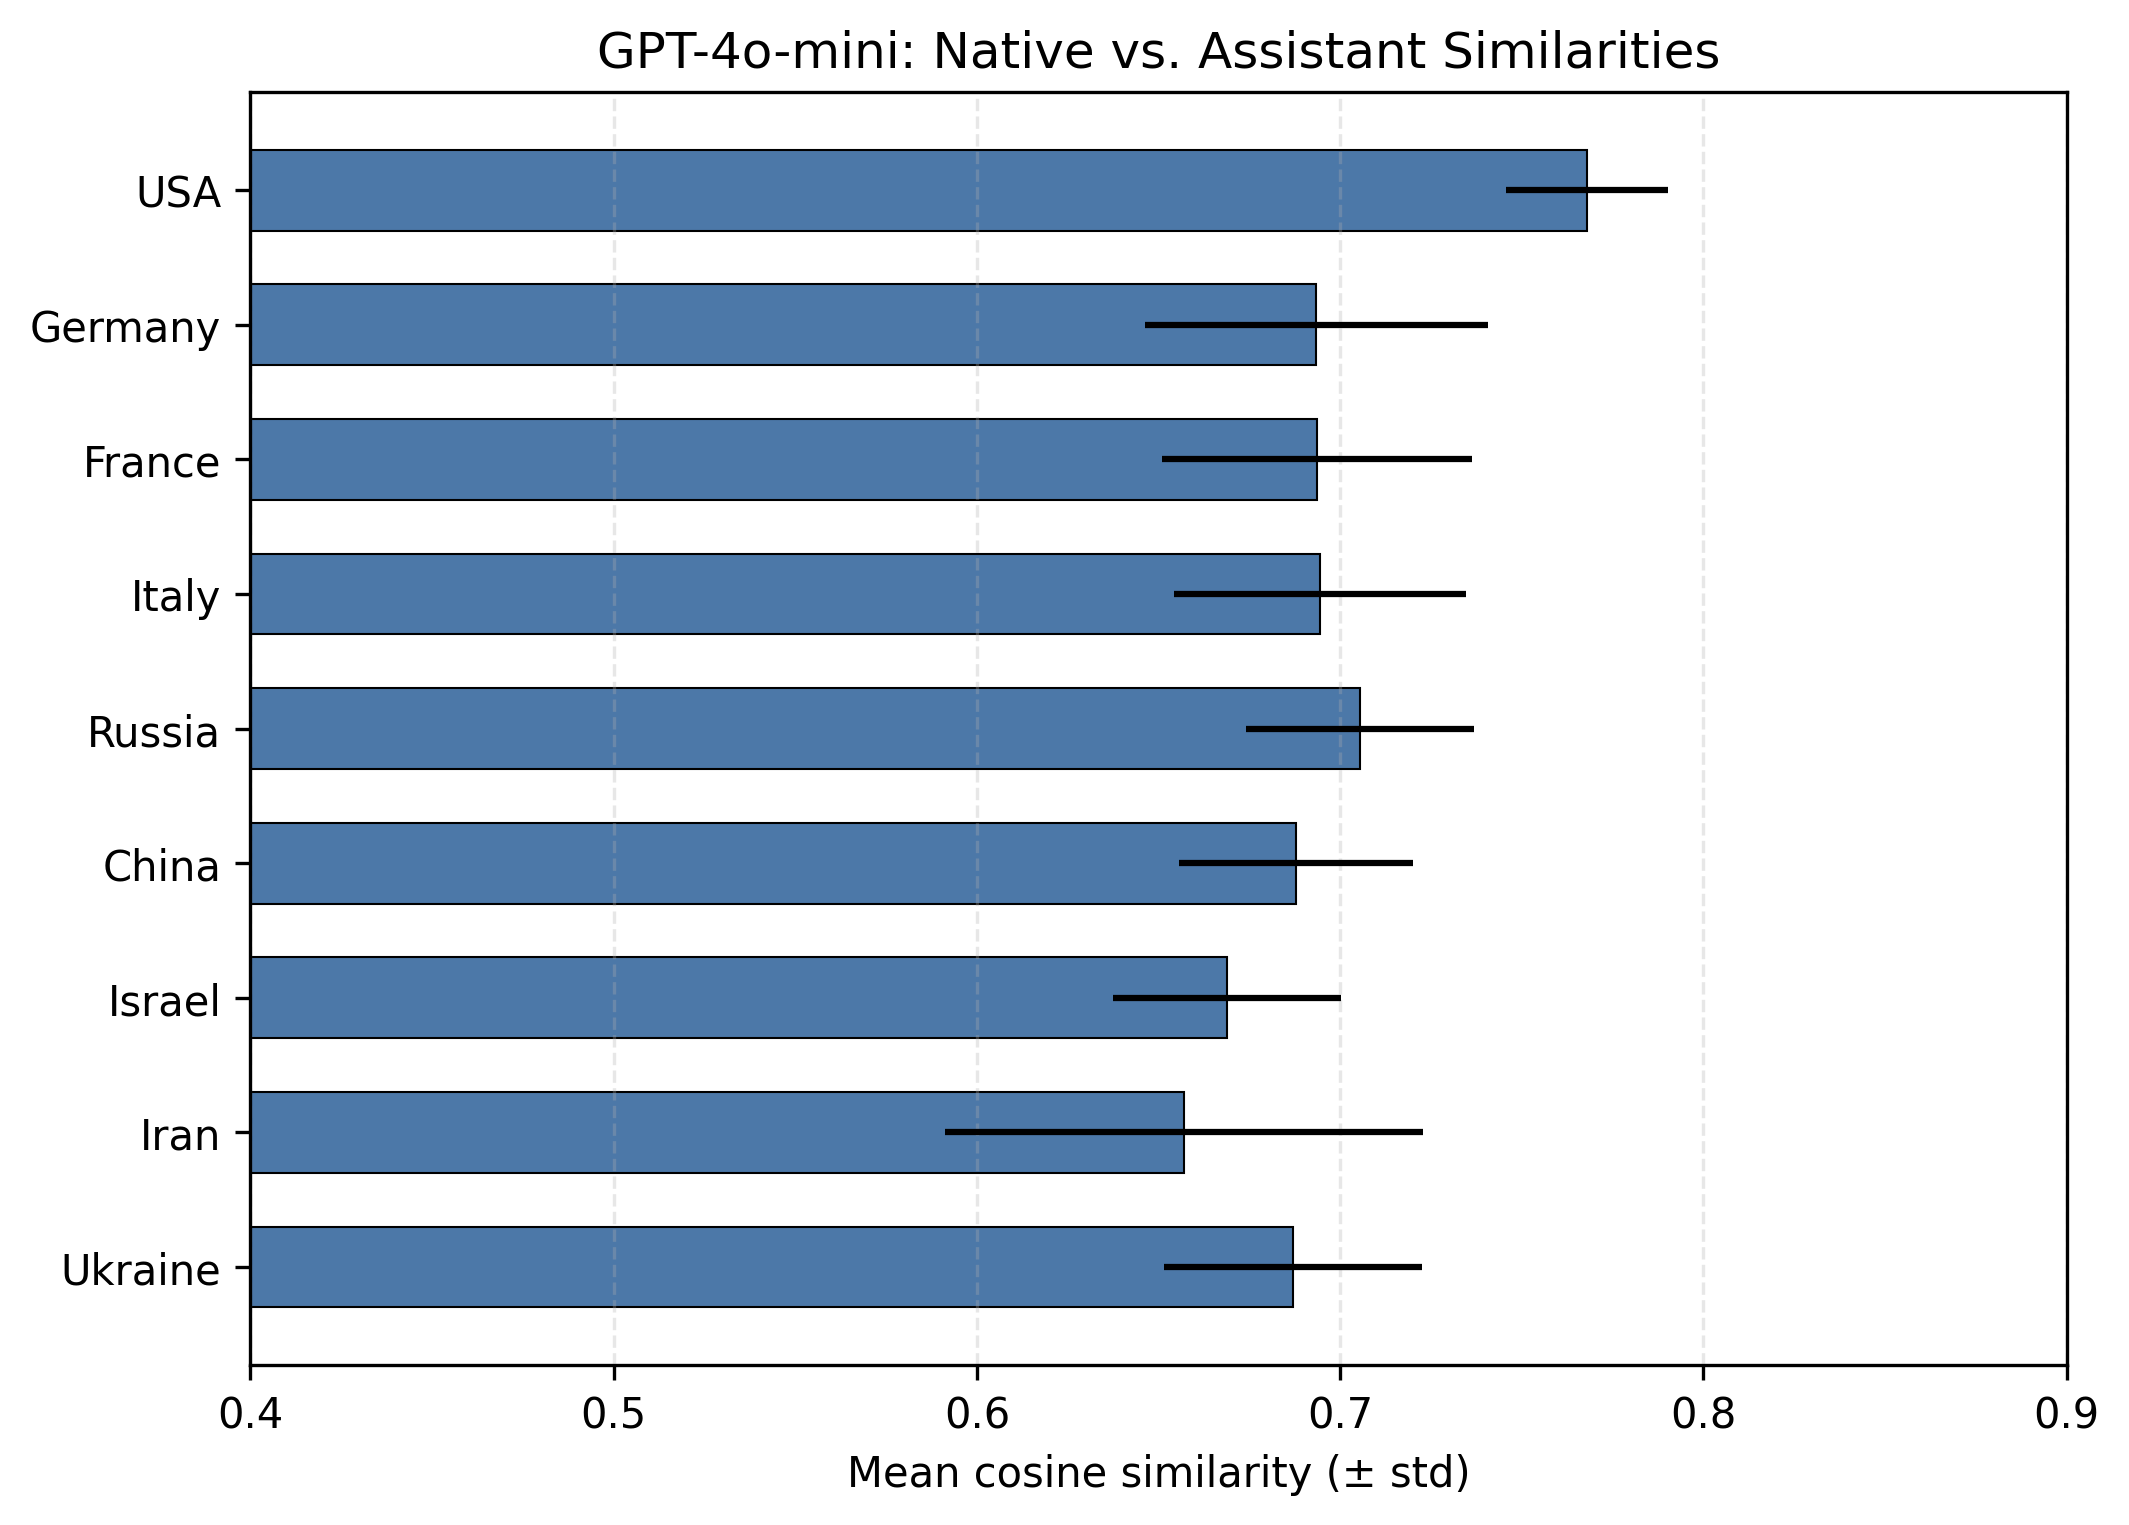
\includegraphics[width=\linewidth]{images/results/similarity/gpt/native_vs_assistant_summary}
    \caption{Native vs. Assistant (NvA)}
  \end{subfigure}
  \caption{\textbf{GPT-4o-mini — mean cosine similarity by country.}
  Bars show means across eight topics; whiskers show \textbf{standard deviation across topics} (topic dispersion).
  NvA and NvR are uniformly high (language and role remain close to native), while RvA is lower and more topic-sensitive (persona effect).}
  \label{fig:gpt_bars}
\end{figure}

\paragraph{Heatmap observations.}
As shown in Figure~\ref{fig:gpt_heat}, across all three comparisons, \textbf{Multi-party system} is among the darkest columns—i.e., highest similarity across countries—and \textbf{Adopt atheism} is also consistently dark. In contrast, \textbf{No economic sanctions}, \textbf{Compulsory voting}, and \textbf{Adopt libertarianism} are repeatedly lighter, especially in the \emph{RvA} heatmap, marking the topics where persona most departs from the assistant baseline. By country, the \textbf{USA} tends to remain dark across topics, while \textbf{China}—and to a lesser extent \textbf{Israel}, \textbf{Iran}, and \textbf{Ukraine}—shows lighter bands in RvA on the low-similarity topics, revealing stronger topic-dependent persona effects.


\begin{figure}[H]
  \centering
  % --- three heatmaps (replace file paths with yours) ---
  \begin{subfigure}{0.75\linewidth}
    \centering
    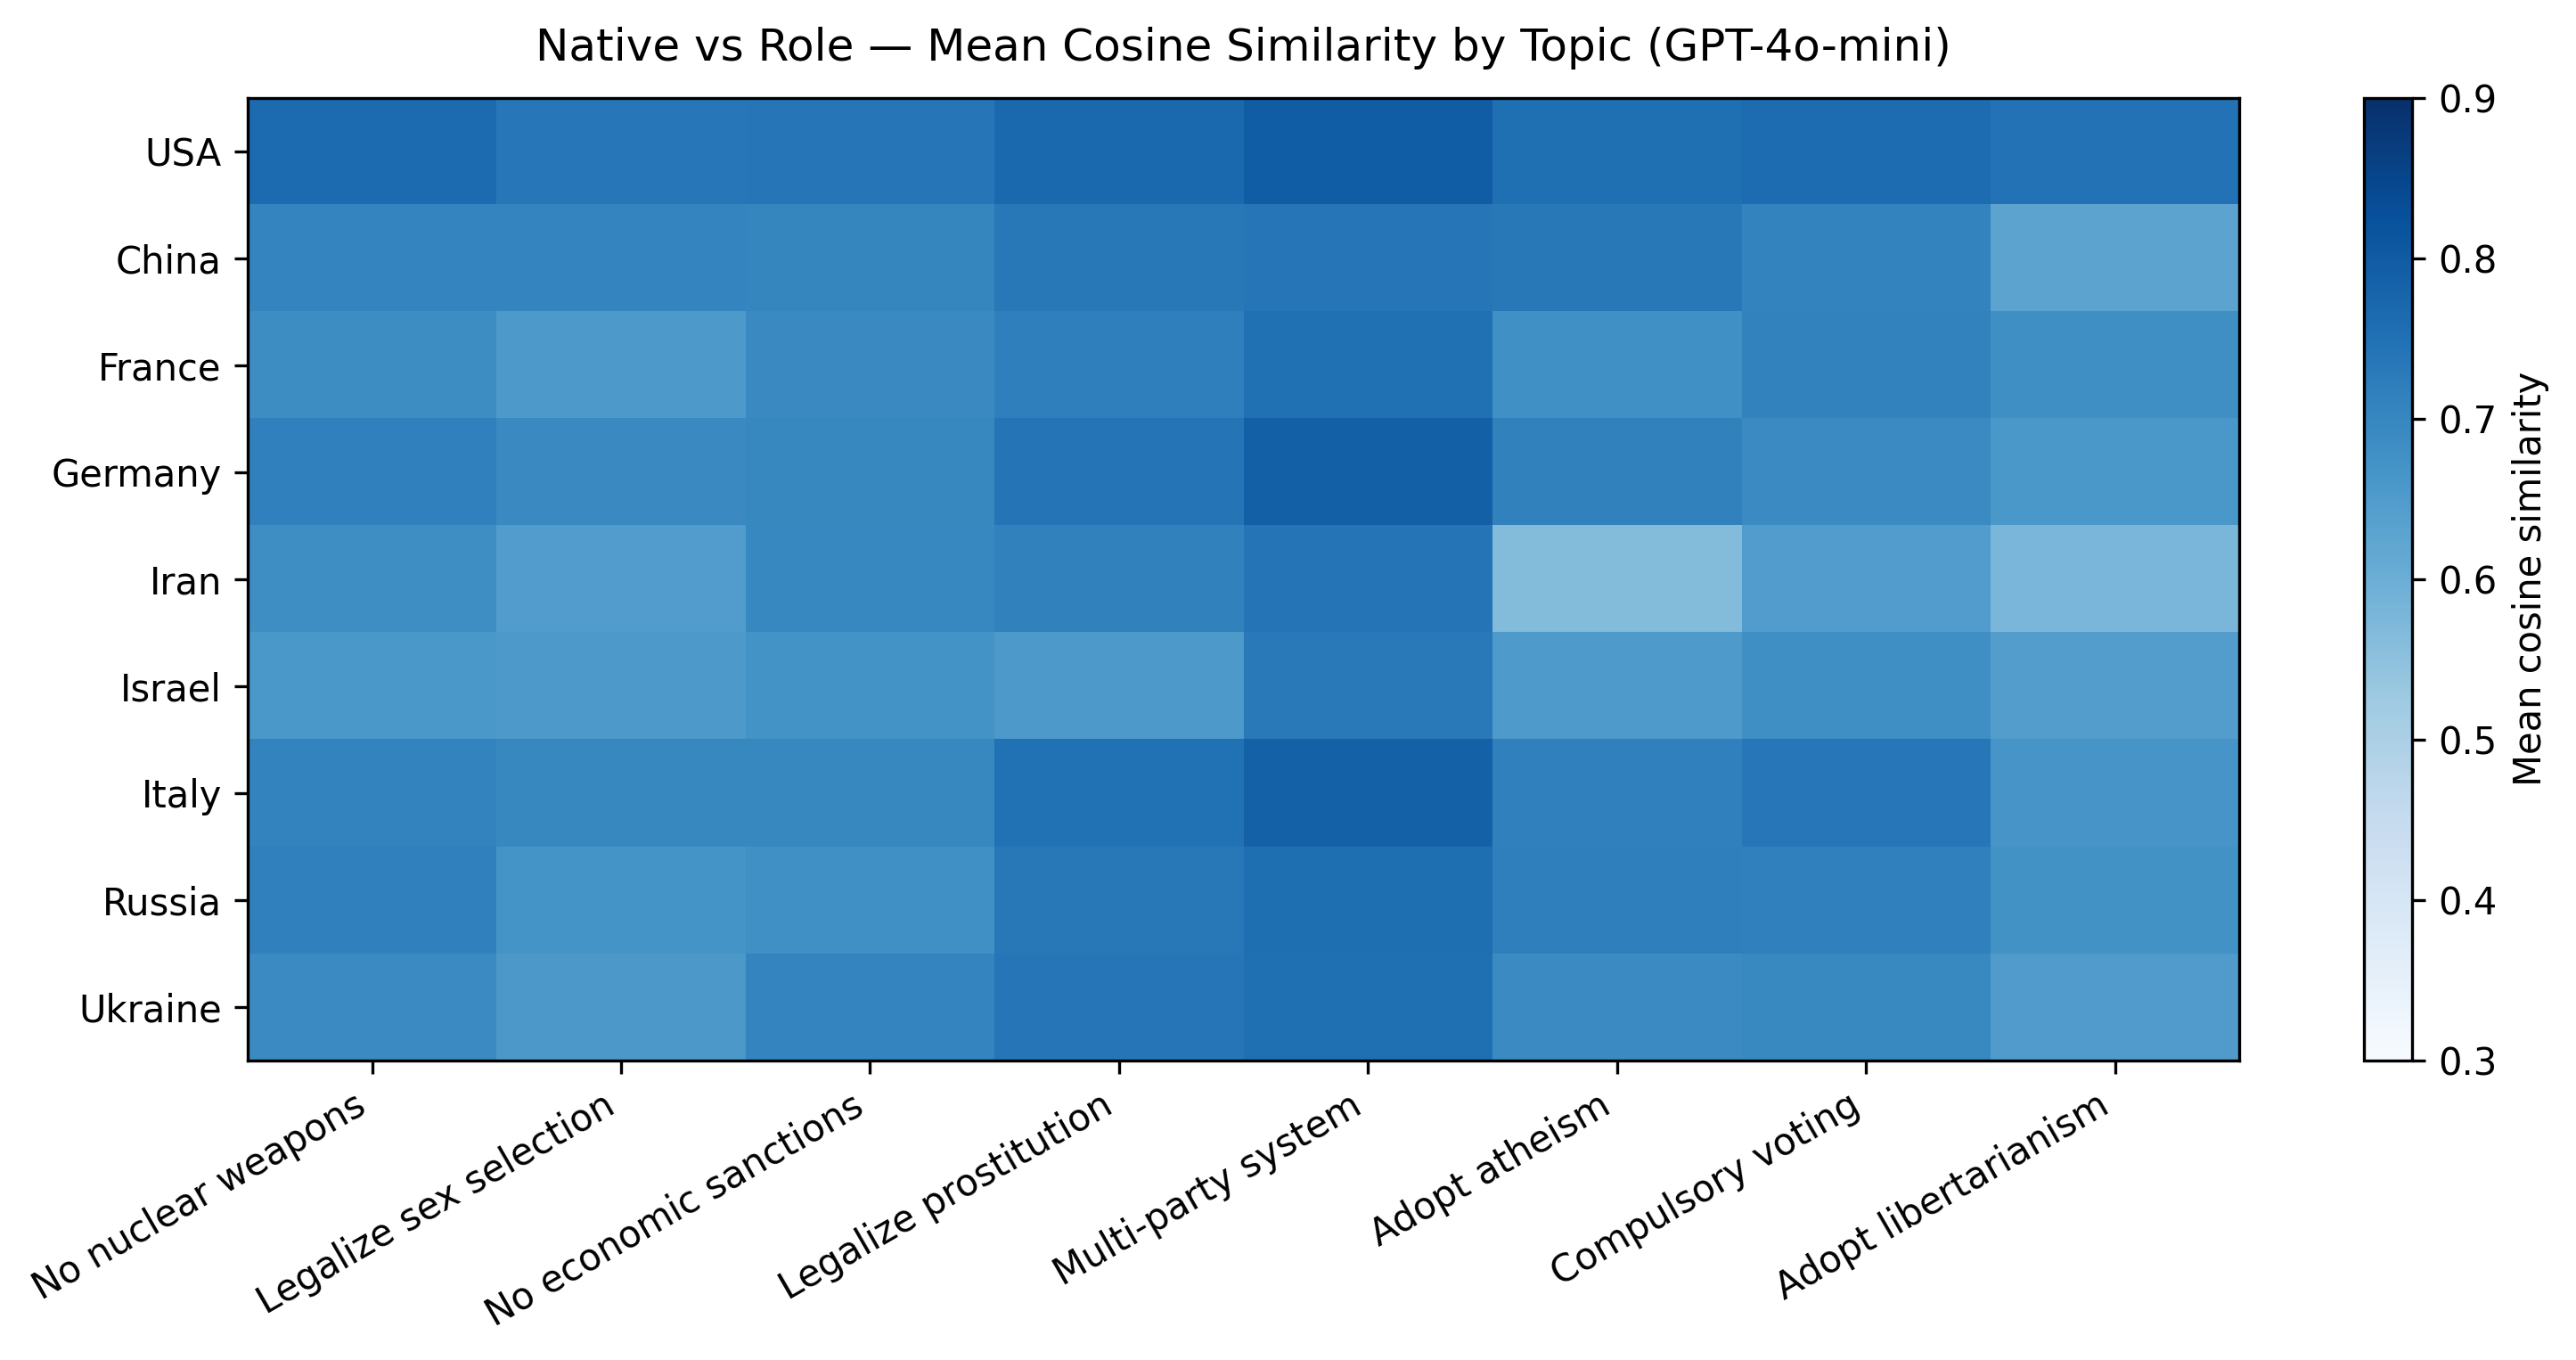
\includegraphics[width=\linewidth]{images/results/similarity/gpt/native_vs_role_heatmap}
    \caption{Native vs. Role (by topic)}
  \end{subfigure}\\[0.5em]
  \begin{subfigure}{0.75\linewidth}
    \centering
    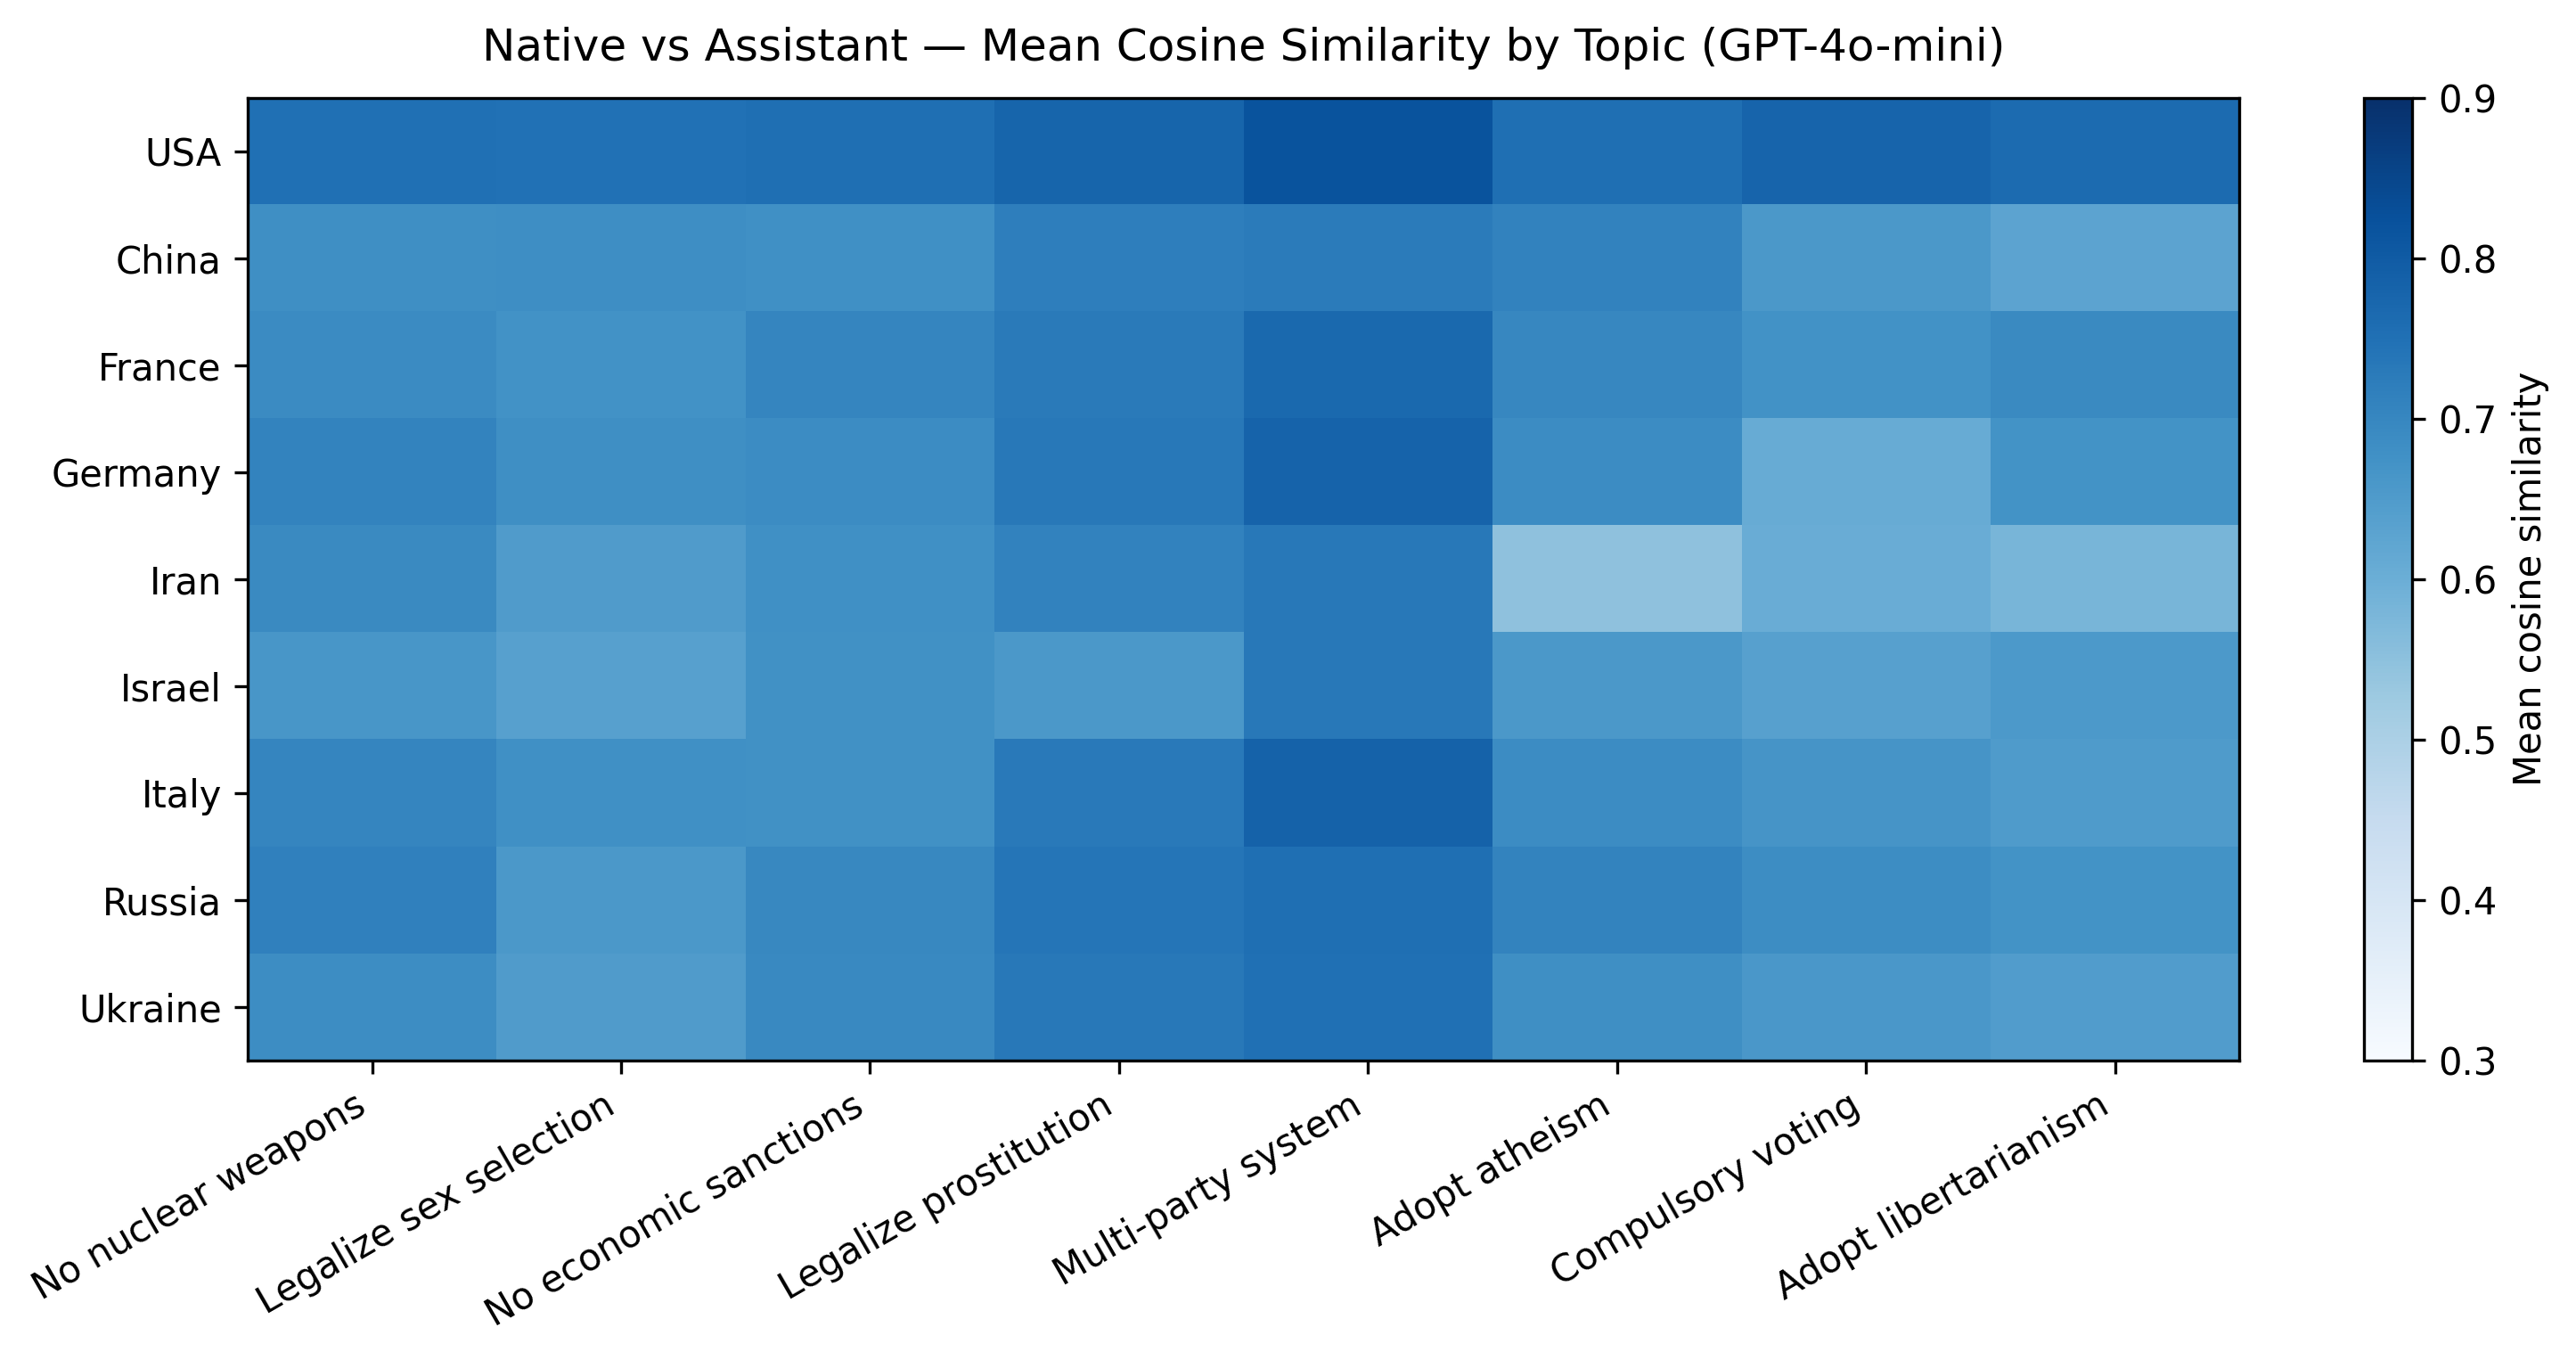
\includegraphics[width=\linewidth]{images/results/similarity/gpt/native_vs_assistant_heatmap}
    \caption{Native vs. Assistant (by topic)}
  \end{subfigure}\\[0.5em]
  \begin{subfigure}{0.75\linewidth}
    \centering
    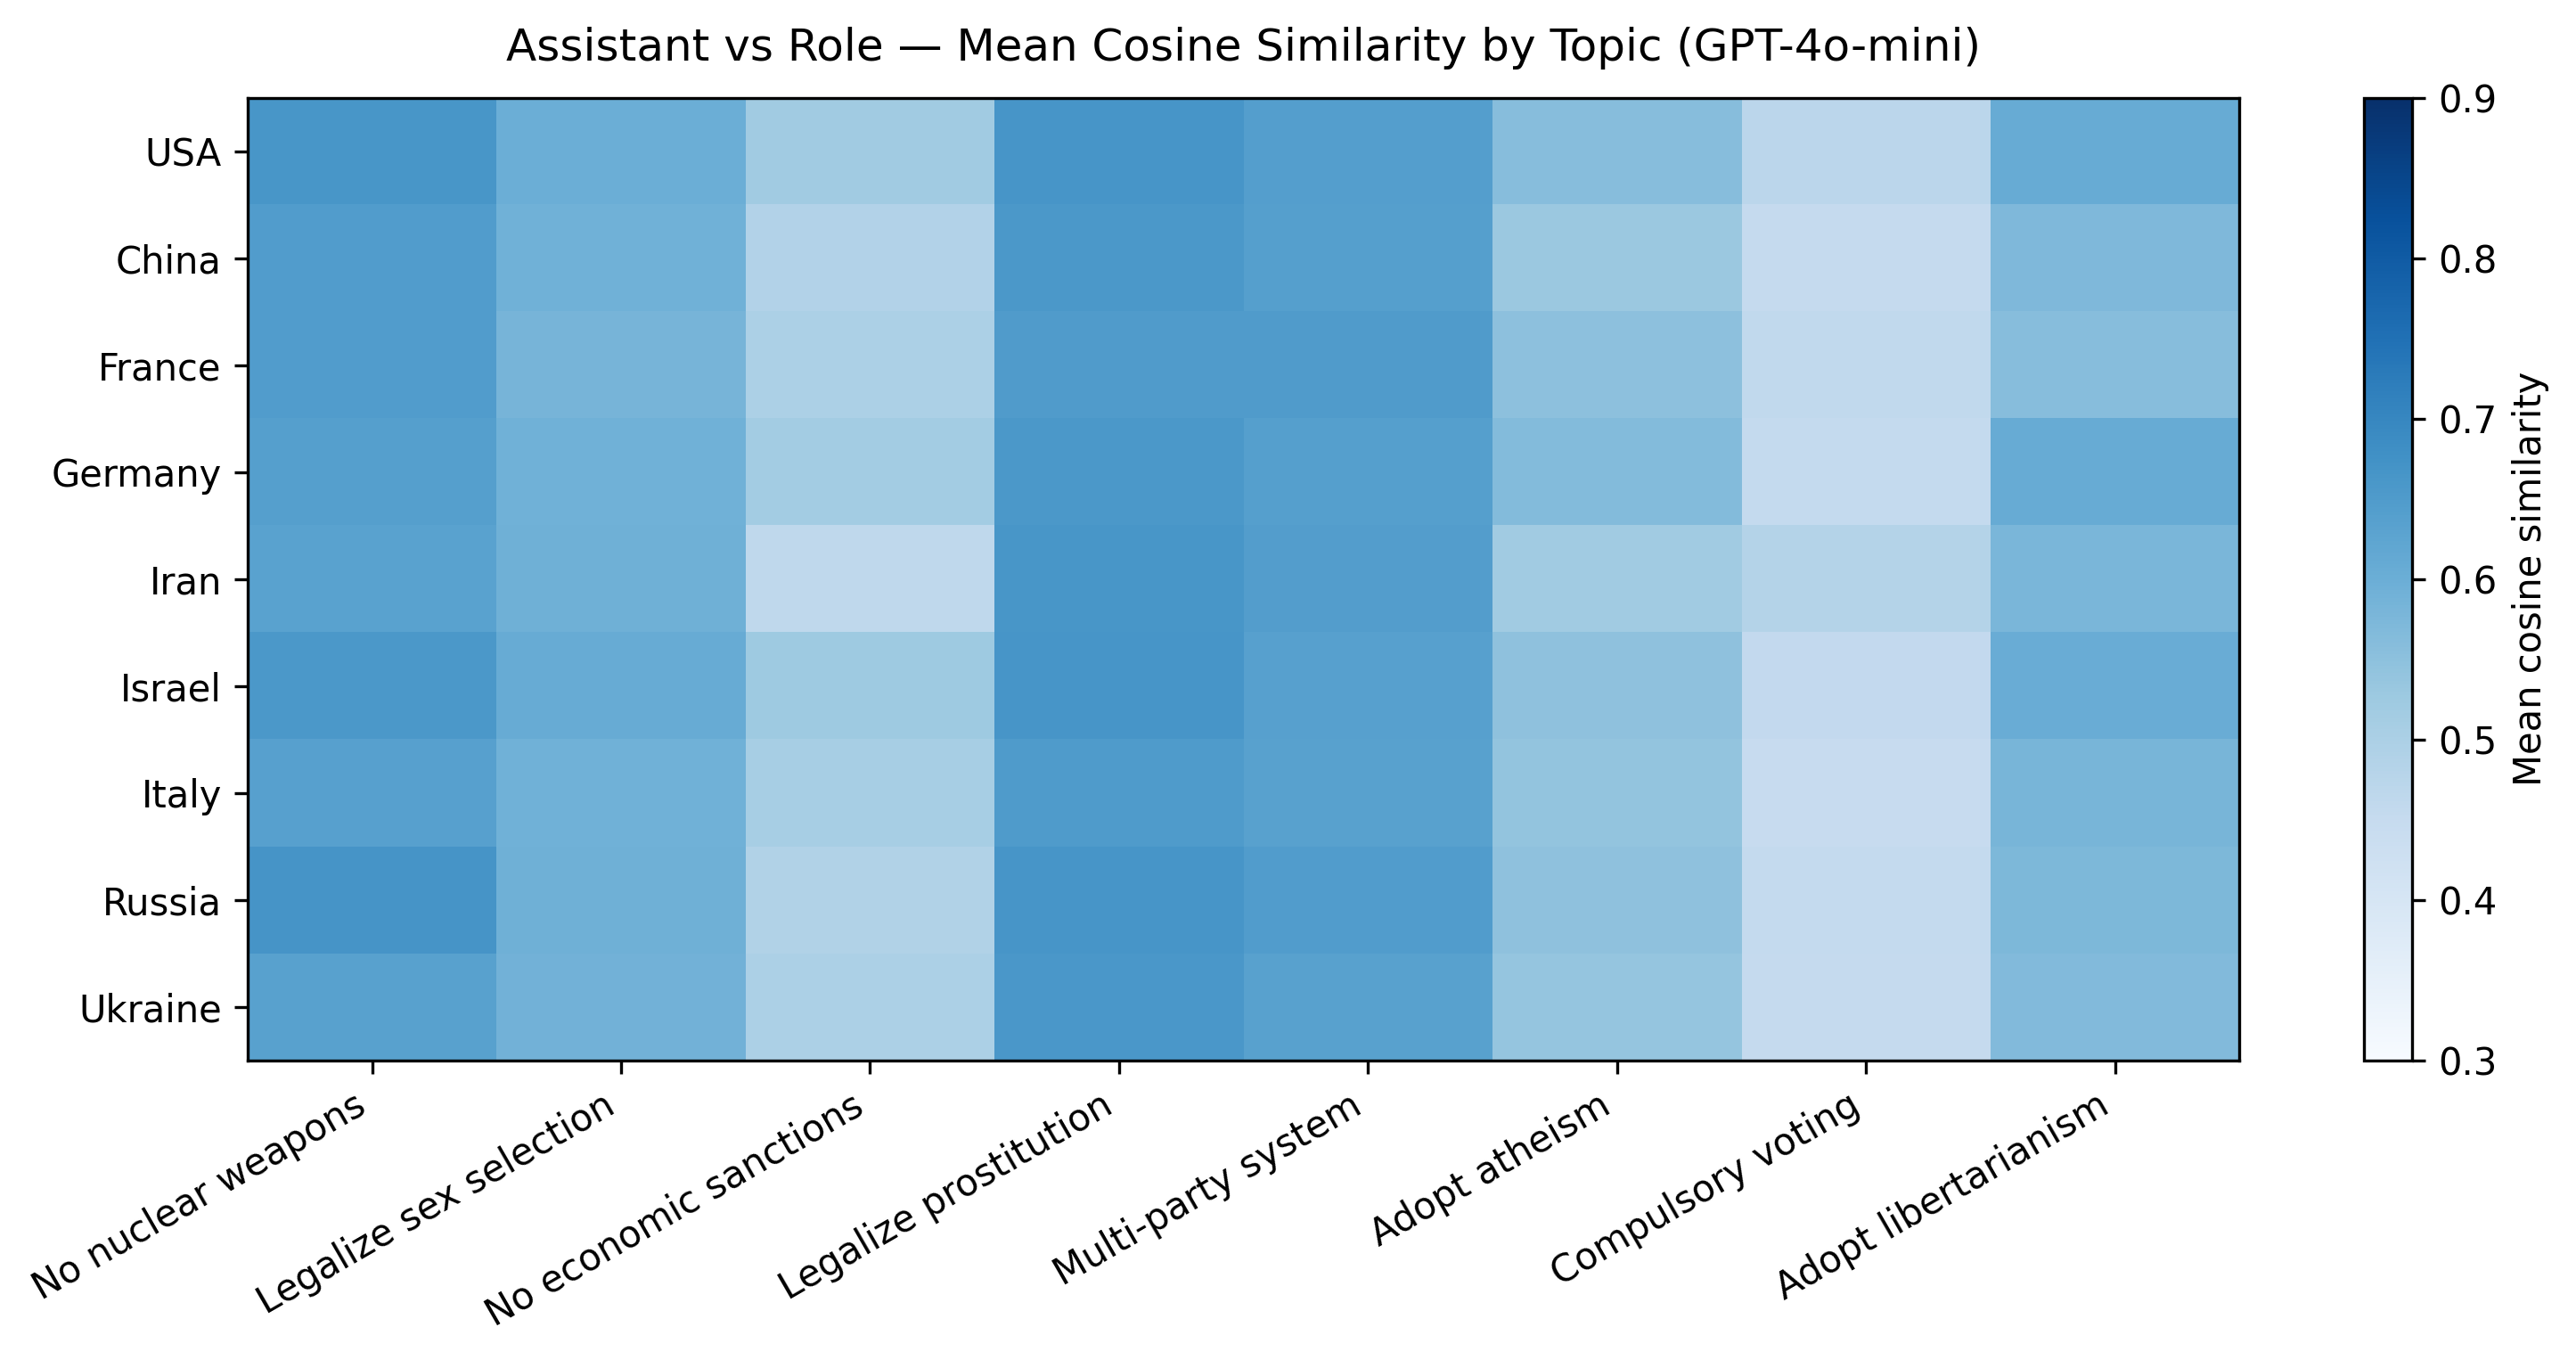
\includegraphics[width=\linewidth]{images/results/similarity/gpt/rolebased_vs_assistant_heatmap}
    \caption{Role vs. Assistant (by topic)}
  \end{subfigure}
  \caption{\textbf{GPT-4o-mini — country–topic heatmaps.}
  Darker cells indicate higher similarity. Most-stable topics (darker across countries) include \emph{Multi-party system} and \emph{Adopt atheism}.
  The lowest rows in RvA (lighter cells) frequently occur on \emph{No economic sanctions}, \emph{Compulsory voting}, and \emph{Adopt libertarianism}, revealing where persona prompts diverge most from the assistant baseline.}
  \label{fig:gpt_heat}
\end{figure}

%---------------------------
\subsection{LLaMA~3.1-70B}
%---------------------------

\paragraph{Bar-chart interpretation.}
As shown in Figure~\ref{fig:llama_bars}, the qualitative picture mirrors GPT-4o-mini. NvA and NvR are high across countries with modest topic dispersion; RvA is visibly lower with the largest dispersion, again strongest for China. Country structure is stable: USA highest and most consistent; France/Italy/Russia/Germany follow; China/Israel/Iran/Ukraine lower and more topic-sensitive in RvA.

\begin{figure}[H]
  \centering
  % --- three bar charts (replace file paths with yours) ---
  \begin{subfigure}{.48\linewidth}
    \centering
    
\includegraphics[width=\linewidth]{images/results/similarity/llama/native_vs_role_summary}
    \caption{Native vs. Role (NvR)}
  \end{subfigure}\hfill
  \begin{subfigure}{.48\linewidth}
    \centering
    
\includegraphics[width=\linewidth]{images/results/similarity/llama/rolebased_vs_assistant_summary}
    \caption{Role vs. Assistant (RvA)}
  \end{subfigure}\\[0.75em]
  \begin{subfigure}{.48\linewidth}
    \centering
    
\includegraphics[width=\linewidth]{images/results/similarity/llama/native_vs_assistant_summary}
    \caption{Native vs. Assistant (NvA)}
  \end{subfigure}
  \caption{\textbf{LLaMA~3.1-70B — mean cosine similarity by country.}
  Bars are means across eight topics; whiskers show \textbf{standard deviation across topics}.
  NvA and NvR remain uniformly high; RvA is lowest with larger topic dispersion, indicating a strong persona effect.}
  \label{fig:llama_bars}
\end{figure}

\paragraph{Heatmap observations.}
As shown in Figure~\ref{fig:llama_heat}, \textbf{Multi-party system} (and often \textbf{Adopt atheism}) forms the darkest columns in NvA/NvR, indicating stable, high similarity of reasons. \textbf{No economic sanctions} is notably light in RvA for several countries, with \textbf{Compulsory voting} and \textbf{Adopt libertarianism} also lighter than other topics—these are the main loci of persona-driven divergence from the assistant. Country-wise, the \textbf{USA} remains dark across many topics, while \textbf{China} shows prominent light bands in RvA on the low-similarity topics; \textbf{Israel}, \textbf{Iran}, and \textbf{Ukraine} also tend to be lighter than the Western European group.

\begin{figure}[H]
  \centering
  \begin{subfigure}{0.75\linewidth}
    \centering
    
\includegraphics[width=\linewidth]{images/results/similarity/llama/native_vs_role_heatmap}
    \caption{Native vs. Role (by topic)}
  \end{subfigure}\\[0.5em]
  \begin{subfigure}{0.75\linewidth}
    \centering
    
\includegraphics[width=\linewidth]{images/results/similarity/llama/native_vs_assistant_heatmap}
    \caption{Native vs. Assistant (by topic)}
  \end{subfigure}\\[0.5em]
  \begin{subfigure}{0.75\linewidth}
    \centering
    
\includegraphics[width=\linewidth]{images/results/similarity/llama/rolebased_vs_assistant_heatmap}
    \caption{Role vs. Assistant (by topic)}
  \end{subfigure}
  \caption{\textbf{LLaMA~3.1-70B — country–topic heatmaps.}
  Darker = higher similarity. As with GPT-4o-mini, \emph{Multi-party system} and \emph{Adopt atheism} are relatively stable/high across countries in NvA/NvR, whereas RvA is lighter on \emph{No economic sanctions}, \emph{Compulsory voting}, and \emph{Adopt libertarianism}, indicating stronger persona-driven divergence.}
  \label{fig:llama_heat}
\end{figure}

\section{Errors and Neutrality}
As shown in Table~\ref{tab:cond_model_error_neutral}, the errors reported here are exclusively due to parsing failures in our pipeline (i.e., cases where the response could not be read as valid JSON). The LLMs themselves successfully generated outputs in all cases, and no generation-level errors were observed.

GPT models did not produce neutral answers in any condition (all neutrality rates are 0). Across the three GPT conditions (Assistant, Native, Role), there was only a single error case in total (Native--GPT: 1/5949, $\approx 0.017\%$), caused by a response that failed JSON parsing. In contrast, LLaMA showed higher error rates (Assistant--LLaMA: 779/5949, $13.0\%$; Role--LLaMA: 871/5949, $14.6\%$; Native--LLaMA: 863/5949, $14.5\%$) and a small but non-zero neutrality rate only in the Native condition (74/5949, $1.2\%$).

\begin{table}[ht]
  \centering
  \label{tab:cond_model_error_neutral}
  \begin{tabular}{lrrrrr}
    \toprule
    \textbf{Condition--Model} & \textbf{Error rate} & \textbf{Neutrality rate} & \textbf{Error count} & \textbf{Neutral count} \\
    \midrule
    Assistant -- GPT   & 0.000 & 0.000 & 0   & 0   \\
    Assistant -- LLaMA & 0.130 & 0.000 & 779 & 0   \\
    Native -- GPT      & 0.000 & 0.000 & 1   & 0   \\
    Native -- LLaMA    & 0.145 & 0.012 & 863 & 74  \\
    Role -- GPT        & 0.000 & 0.000 & 0   & 0   \\
    Role -- LLaMA      & 0.146 & 0.000 & 871 & 0   \\
    \bottomrule
  \end{tabular}
  \caption{Error and neutrality summary across condition--model pairs. Error rate is computed as \textit{error\_count}/\textit{total\_rows}; neutrality rate as \textit{neutral\_count}/\textit{total\_rows}.}
\end{table}

